%% Copyright (C) 2015 Quang-Cuong Pham <cuong.pham@normalesup.org>
%% This work is licensed under the Creative Commons
%% Attribution-NonCommercial-ShareAlike 4.0 International License. To
%% view a copy of this license, visit
%% http://creativecommons.org/licenses/by-nc-sa/4.0/.


%TODO
% pole/zero compensation
% PI control by system type (do not re-derive the results)
% Lead compensator design by algebraic method
% Explain poles vs poles
% Figure slow convergence




\documentclass[a4paper,11pt]{report}

\usepackage{mathtools}
%\documentclass[preprint,12pt]{elsarticle}
\usepackage{adjustbox}
%\usepackage[utf8]{inputenc}
\usepackage{amsmath}
%\usepackage{accents}
\usepackage{amssymb}
\usepackage{graphicx}
%\usepackage{natbib}
\usepackage{setspace}
%\doublespacing
%XXXX
%\setstretch{1.4}
\usepackage{hyperref}
\usepackage{amsthm}
\theoremstyle{definition}


\usepackage{xcolor}
\usepackage{mdframed}


\usepackage{tikz}
\usetikzlibrary{positioning}
\usetikzlibrary{shapes,arrows} 

\usepackage{mathrsfs}
\usepackage{float}

\usepackage{chngcntr}
\counterwithin{figure}{chapter}

\newcommand{\defeq}{\stackrel{\mathrm{def}}{=}}

\newcommand{\ud}{\mathrm{d}}

\newcommand{\bfa}{\mathbf{a}}
\newcommand{\bfb}{\mathbf{b}}
\newcommand{\bfc}{\mathbf{c}}
\newcommand{\bfd}{\mathbf{d}}
\newcommand{\bfe}{\mathbf{e}}
\newcommand{\bff}{\mathbf{f}}
\newcommand{\bfg}{\mathbf{g}}
\newcommand{\bfh}{\mathbf{h}}
\newcommand{\bfk}{\mathbf{k}}
\newcommand{\bfm}{\mathbf{m}}
\newcommand{\bfu}{\mathbf{u}}
\newcommand{\bfv}{\mathbf{v}}
\newcommand{\bfx}{\mathbf{x}}
\newcommand{\bfy}{\mathbf{y}}
\newcommand{\bfz}{\mathbf{z}}

\newcommand{\bfA}{\mathbf{A}}
\newcommand{\bfB}{\mathbf{B}}
\newcommand{\bfC}{\mathbf{C}}
\newcommand{\bfE}{\mathbf{E}}
\newcommand{\bfF}{\mathbf{F}}
\newcommand{\bfG}{\mathbf{G}}
\newcommand{\bfH}{\mathbf{H}}
\newcommand{\bfI}{\mathbf{I}}
\newcommand{\bfJ}{\mathbf{J}}
\newcommand{\bfK}{\mathbf{K}}
\newcommand{\bfL}{\mathbf{L}}
\newcommand{\bfM}{\mathbf{M}}
\newcommand{\bfP}{\mathbf{P}}
\newcommand{\bfQ}{\mathbf{Q}}
\newcommand{\bfR}{\mathbf{R}}
\newcommand{\bfT}{\mathbf{T}}
\newcommand{\bfU}{\mathbf{U}}
\newcommand{\bfV}{\mathbf{V}}
\newcommand{\bfW}{\mathbf{W}}
\newcommand{\bbC}{\mathbb{C}}
\newcommand{\bbR}{\mathbb{R}}


\newcommand{\bfTh}{\mathbf{\Theta}}
\newcommand{\zeros}{\mathbf{0}}
\newcommand{\sM}{\mathcal{M}}

\newcommand{\dm}[1]{d_{\mathbf{M}(#1)}}
\newcommand{\tr}{\mathrm{tr}}
\newcommand{\lift}{\mathrm{lift}}
\newcommand{\re}{\mathrm{ref}}

\newcommand{\expect}{\mathbb{E}}
\newcommand{\expectx}{\mathbb{E}_{\bfx}}
\newcommand{\proba}{\mathbb{P}}
\newcommand{\des}{\textrm{desired}}
\newcommand{\defi}{\mathrm{def}}
\newcommand{\sse}{\mathrm{ss}}

% %%%%debutmacro%%%%
% \makeatletter
% \renewcommand\theequation{\thesection.\arabic{equation}}
% \@addtoreset{equation}{section}
% \makeatother
% %%%%finmacro%%%%

\newcommand{\bffg}{\accentset{\frown}{\mathbf{f}}}
\newcommand{\bfxg}{\accentset{\frown}{\mathbf{x}}}
\newcommand{\bfyg}{\accentset{\frown}{\mathbf{y}}}
\newcommand{\sg}{\accentset{\frown}{\sigma}}
\newcommand{\Sg}{\accentset{\frown}{S}}
\newcommand{\zg}{\accentset{\frown}{z}}


\newtheorem{prop}{Proposition}
\newtheorem{theorem}{Theorem}
\newtheorem{corollary}{Corollary}
\newtheorem{definition}{Definition}
%\newtheorem{example}{Example}

\definecolor{lightgray}{rgb}{0.9, 0.9, 0.9}
\definecolor{lightgray2}{rgb}{0.8, 0.8, 0.8}
\newtheorem{mdexample}{Example}
\newenvironment{example}%
  {\vspace{0.1cm}\begin{mdframed}[backgroundcolor=lightgray]\begin{mdexample}}%
  {\end{mdexample}\end{mdframed}\vspace{0.1cm}}

\newtheorem{mdinsight}{Insight}
\newenvironment{insight}%
  {\vspace{0.1cm}\begin{mdframed}[backgroundcolor=lightgray2]\begin{mdinsight}
        \begingroup
        \fontsize{9pt}{11pt}\selectfont
      }%
  {\endgroup\end{mdinsight}\end{mdframed}\vspace{0.1cm}}


\newtheorem{mdsummary}{Summary}
\newenvironment{summary}%
  {\vspace{0.1cm}\begin{mdframed}[linecolor=red!60!black,
  linewidth=2pt]\begin{mdsummary}}%
  {\end{mdsummary}\end{mdframed}\vspace{0.1cm}}

\title{Control Theory MA3005\\Part II\,: Controller design}
\author{Quang-Cuong Pham\\
  School of Mechanical and Aerospace Engineering\\ 
  Nanyang Technological University, Singapore}


\begin{document}

\maketitle

\paragraph{Disclaimer} These notes are provided to help the students of
MA3005 get a more systematic understanding of the topics presented
during the lecture. I assume no liability or responsibility for any
errors or omissions in the content. Students are advised to refer to
the live lecture and lecture slides for exam-related matters.

\tableofcontents

\setcounter{chapter}{-1}

\chapter{Recapitulation of part I}

\section{Stability and transient behavior}

\subsection{Characteristic equation and stability}

The stability of a system is determined by the \emph{denominator} of
the transfer function, which is also called the \emph{Characteristic
  Equation} (CE). More precisely, it is determined by the locations of
the roots of the CE -- also called \emph{poles} -- in the complex
plane.

\begin{itemize}
  \item If all the poles are in the open left half-plane,
    the system is \emph{stable}, see Fig.~\ref{fig:ex-stable};
  \item If all the poles are in the closed left half-plane, and a pair
    of roots are on the imaginary axis, the system is \emph{marginally
      stable}, see Fig.~\ref{fig:ex-margstable};
  \item If at least one pole is in the open right half-plane, the
    system is \emph{unstable}, see Fig.~\ref{fig:ex-unstable}.
\end{itemize}

\begin{figure}[H]
  \centering
  \noindent System poles \hspace{2cm} Response to unit step

  \vspace{0.2cm}
  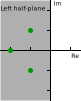
\includegraphics[height=5cm]{fig/stability.pdf}
  \includegraphics[height=5cm]{fig/sys-stable.pdf}
  \caption{A stable system with transfer function
    $\frac{C}{R}=\frac{1}{s^3+4s^2+6s+4}$. The CE is $s^3+4s^2+6s+4$,
    which has three roots: $-1\pm j, -2$.}
  \label{fig:ex-stable}
\end{figure}

\begin{figure}[H]
  \centering
  \noindent System poles \hspace{2cm} Response to unit step

  \vspace{0.2cm}
  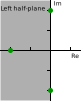
\includegraphics[height=5cm]{fig/stability-marg.pdf}
  \includegraphics[height=5cm]{fig/sys-margstable.pdf}
  \caption{A marginally stable system with transfer function
    $\frac{C}{R}=\frac{1}{s^3+2s^2+4s+8}$. The CE is $s^3+2s^2+4s+8$,
    which has three roots: $\pm 2j, -2$. The frequency of oscillation
    is given by $\omega$, where $\omega$ is the norm of the roots on
    the imaginary axis (here $\omega=2$\,rad/s).}
  \label{fig:ex-margstable}
\end{figure}

\begin{figure}[H]
  \centering
  \noindent System poles \hspace{2cm} Response to unit step

  \vspace{0.2cm}
  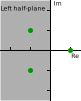
\includegraphics[height=5cm]{fig/stability-no.pdf}
  \includegraphics[height=5cm]{fig/sys-unstable.pdf}
  \caption{An unstable system with transfer function
    $\frac{C}{R}=\frac{1}{s^3+s^2-2}$. The CE is $s^3+s^2-2$,
    which has three roots: $-1\pm j, 1$.}
  \label{fig:ex-unstable}
\end{figure}


\subsection{Transient behavior}

Once a system has been determined as stable, one can investigate its
transient behavior, roughly, how fast does the system response
converge to its final value. This is measured by quantities such as
settling time or maximum overshoot.

The transient behavior depends primarily on the precise location of
the dominant (i.e. rightmost) poles in the complex plane. The further
the dominant poles to the left, the faster the convergence (the
smaller the settling time and the maximum overshoot). Compare
Fig.~\ref{fig:convergence-comp}, red line and
Fig.~\ref{fig:convergence-comp}, green line : both systems are stable,
but the red system converges faster than the green system, since its
dominant poles are located more to the left ($-2\pm j$ vs $-1\pm
j$).

\begin{figure}[H]
  \includegraphics[height=8cm]{fig/convergence-comp.pdf}
  \caption{Comparison of the convergence speed of two systems. Red:
    unit-step response of a system with transfer function
    $\frac{C}{R}=\frac{5}{s^2+4s+5}$. The CE is $s^2+4s+5$, which has
    two roots: $-2\pm j$. Green: unit-step response of a system with
    transfer function $\frac{C}{R}=\frac{2}{s^2+2s+2}$. The CE is
    $s^2+2s+2$, which has two roots: $-1\pm j$.}
  \label{fig:convergence-comp}
\end{figure}


The transient behavior (in particular, whether the system oscillates,
etc.) is also affected by other quantities such as the damping ratio
$\zeta$ and the undamped natural frequency $\omega_0$. For more
details, refer to the slides from Part I of the course.

\section{Steady-state error}

\subsection{Definition}

Consider a feedback system as in Fig.~\ref{fig:sse}.

\begin{figure}[H]
  \centering
  \tikzstyle{block} = [draw, fill=blue!20, rectangle, minimum height=3em, minimum width=4em]
  \tikzstyle{block2} = [draw, fill=blue!20, rectangle, minimum height=2em, minimum width=2em]
  \tikzstyle{sum} = [draw, fill=blue!20, circle, node distance=1cm]
  \tikzstyle{input} = [coordinate]
  \tikzstyle{output} = [coordinate]
  \begin{tikzpicture}[auto, >=latex']
    % Nodes
    \node [input] (input) {};
    \node [sum, right = 1cm of input] (sum) {};
    %\node [block2, right = 1cm of sum] (system) {$K$};
    \node [block, right = 1cm of sum] (system2) {$G$};
    \node [output, right = 2cm of system2] (output) {};
    \node [block, below = 0.5cm of system2] (h) {$H$};
    % Arrows
    \draw [draw,->] (input) -- node {$R$} (sum);
    \draw [->] (sum) -- node {$E$} (system2);
    %\draw [->] (system) -- (system2);
    \draw [->] (system2) -- node (y) {$C$}(output);
    \draw [-] (y) |- (h) {} ;
    \draw [->] (h) -| node[pos=0.99] {$-$}  node [near end] {} (sum);
  \end{tikzpicture}  
  \caption{Error signal: $E=R-C$}
  \label{fig:sse}
\end{figure}

The steady-state error (if it exists) is defined by
\begin{equation}
  \label{eq:sse}
  e_\sse := \lim_{t\to\infty} e(t).
\end{equation}

If the system is stable, one can apply the Finaly Value Theorem to obtain
\[
\lim_{t\to\infty} e(t) = \lim_{s\to 0} sE(s).
\]

In general, one would like the steady-state error to be as small as
possible, ideally zero.

\subsection{System type and steady-state error}

In general, to calculate the steady-state error, one uses the FVT as
in equation~(\ref{eq:sse}). However, if the system is stable and
\emph{unity-feedback}, then one can determine the system type and use
this information to obtain the steady-state error much more easily.

Let $G$ be the feedforward transfer function. Assume that $G$ is
written as
\[
G=\frac{N(s)}{s^kD(s)},
\]
where $N$ and $D$ are not factorizable by $s$. Then the type of the
system is given by the integer $k$. Fig.~\ref{fig:systype} shows the
general form of systems of types 1, 2 and 3.

\begin{figure}[H]
  \hspace{1.5cm}\textbf{Type 0}\hspace{3cm}\textbf{Type
    1}\hspace{3cm}\textbf{Type 2}\\
  \vspace{0.1cm} 

  \centering \tikzstyle{block} = [draw, fill=blue!20,
  rectangle, minimum height=3em, minimum width=3em]
  \tikzstyle{controller} = [draw, fill=red!20, rectangle, minimum
  height=3em, minimum width=4em] \tikzstyle{sum} = [draw,
  fill=blue!20, circle, node distance=1cm] \tikzstyle{input} =
  [coordinate] \tikzstyle{output} = [coordinate]
  \begin{tikzpicture}[auto, >=latex']
    % Nodes
    \node [input] (input) {};
    \node [sum, right = 0.5cm of input] (sum) {};
    \node [block, right = 0.5cm of sum] (system) {$\frac{N_0(s)}{D_0(s)}$};
    \node [output, right = 1cm of system] (output) {};
    \node [input, below = 0.5cm of system] (m) {};
    % Arrows
    \draw [draw,->] (input) -- node {$R$} (sum);
    \draw [->] (sum) -- node {} (system);
    \draw [->] (system) -- node (y) {$C$}(output);
    \draw [-] (y) |- (m) {} ;
    \draw [->] (m) -| node[pos=0.99] {$-$}  node [near end] {} (sum);
  \end{tikzpicture}  
  \hspace{0.5cm}
  \begin{tikzpicture}[auto, >=latex']
    % Nodes
    \node [input] (input) {};
    \node [sum, right = 0.5cm of input] (sum) {};
    \node [block, right = 0.5cm of sum] (system) {$\frac{N_1(s)}{sD_1(s)}$};
    \node [output, right = 1cm of system] (output) {};
    \node [input, below = 0.5cm of system] (m) {};
    % Arrows
    \draw [draw,->] (input) -- node {$R$} (sum);
    \draw [->] (sum) -- node {} (system);
    \draw [->] (system) -- node (y) {$C$}(output);
    \draw [-] (y) |- (m) {} ;
    \draw [->] (m) -| node[pos=0.99] {$-$}  node [near end] {} (sum);
  \end{tikzpicture}  
  \hspace{0.5cm}
  \begin{tikzpicture}[auto, >=latex']
    % Nodes
    \node [input] (input) {};
    \node [sum, right = 0.5cm of input] (sum) {};
    \node [block, right = 0.5cm of sum] (system) {$\frac{N_2(s)}{s^2D_2(s)}$};
    \node [output, right = 1cm of system] (output) {};
    \node [input, below = 0.5cm of system] (m) {};
    % Arrows
    \draw [draw,->] (input) -- node {$R$} (sum);
    \draw [->] (sum) -- node {} (system);
    \draw [->] (system) -- node (y) {$C$}(output);
    \draw [-] (y) |- (m) {} ;
    \draw [->] (m) -| node[pos=0.99] {$-$}  node [near end] {} (sum);
  \end{tikzpicture}  
  \caption{Systems of types 0, 1 and 2. Note that $N_0, N_1, N_2, D_0,
    D_1, D_2$ should not be factorizable by $s$.}
  \label{fig:systype}
\end{figure}

Let us carry further the computation of the steady-state error for a
stable unity-feedback system.
\[
sE(s) = s(R(s)-C(s)) = s\left(R(s)-\frac{G(s)}{1+G(s)}R(s)\right)=\frac{s}{1+G(s)}R(s).
\]

For unit-step input, one has $R(s)=1/s$. Thus,
\[
sE(s) = \frac{s}{1+G(s)}*\frac{1}{s} = \frac{1}{1+G(s)}
\xrightarrow[s\to 0]{}\frac{1}{1+\lim_{s\to 0}G(s)}.
\]
For a system of type 0, one has
\[
\lim_{s\to 0}G(s) = \lim_{s\to 0}\frac{N_0(s)}{D_0(s)} = \frac{N_0(0)}{D_0(0)}.
\]
Thus, the steady-state error of a system of type 0 for unit-step input
is given by
\[
e_\sse = \frac{1}{1+\frac{N_0(0)}{D_0(0)}}.
\]

Carrying out similar calculations, one obtains the following table,
which shows the steady-state errors of systems of types 0, 1, 2, 3 for
unit-step, unit-ramp and unit-parabola inputs.

\begin{table}[htp]
  \centering
  \begin{tabular}{|c|c|c|c|}
    \hline
    System type&Step input&Ramp input&Parabolic input\\\hline
    Type 0&$\frac{1}{1+K_p}$&$\infty$&$\infty$\\\hline
    Type 1&0&$\frac{1}{K_v}$&$\infty$\\\hline
    Type 2&0&0&$\frac{1}{K_a}$\\\hline
    Type 3&0&0&0\\\hline
  \end{tabular}
  \caption{Steady-state errors of systems of different types and for
    different inputs.}
  \label{tab:systype}
\end{table}

The constants $K_p$, $K_v$, and $K_a$ are defined as below
\begin{itemize}
\item for a system of type 0, $K_p:=\frac{N_0(0)}{D_0(0)}$ (position constant);
\item for a system of type 1, $K_v:=\frac{N_1(0)}{D_1(0)}$ (velocity constant);
\item for a system of type 2, $K_a:=\frac{N_2(0)}{D_2(0)}$
  (acceleration constant).
\end{itemize}

\begin{example}
  Consider a unity-feedback system with feedforward transfer function
  \[
  G(s) = \frac{s^2+2s}{2s^4+s^3+3s^2}.
  \]
  What is the steady-state error of the system for unit-ramp and
  unit-parabola inputs?

  Answer: One can simplify $G$ as follows
  \[
  G(s) = \frac{s(s+2)}{s^2(2s^2+s+3)} =  \frac{s+2}{s(2s^2+s+3)},
  \]
  which implies that the system is of type 1, with 
  \[
  N(s) = s+2 \quad ; \quad D(s) = 2s^2+s+3.
  \]
  From the table, the steady-state error for unit-ramp input is given
  by
  \[
  e_\sse=\frac{1}{K_v},
  \]
  where the velocity constant $K_v$ is given by
  \[
  K_v = \frac{N(0)}{D(0)} = \frac{2}{3}.
  \]
  Thus $e_\sse = 1.5$.

  Also from the table, the steady-state error for unit-parabola input
  is $\infty$.
\end{example}

\chapter{Introduction to controller design}

\section{A simple controller design problem}

\subsection{Problem setting}

Consider the helicopter in Fig.~\ref{fig:helico}. Applying Newton's
second law in the vertical axis, we obtain
\begin{equation}
  \label{eq:quaddyn0}
  m\ddot z = F_\lift - mg,  
\end{equation}
where $g=9.81$\,m$\cdot$s$^{-1}$ is the gravitational coefficient.

\begin{figure}[H]
  \centering
  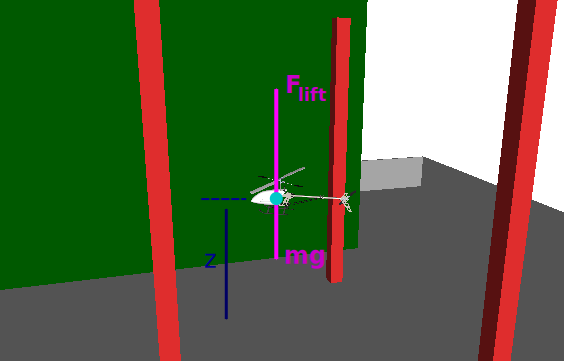
\includegraphics[width=10cm]{fig/helico.pdf}
  \caption{A helicopter.}
  \label{fig:helico}
\end{figure}


The lift force $F_\lift$ is proportional to the rotor speed
$\omega_\textrm{rotor}$, which is in turn proportional to the electric
current $i_\textrm{rotor}$ fed into the motor. One can thus write
\[
F_\lift = k i_\textrm{rotor},
\]
where $k$ is a positive constant.

To eliminate the constant term $mg$, let us note $i=
i_\textrm{rotor}-\frac{mg}{k}$. Equation~(\ref{eq:quaddyn0}) becomes
\begin{equation}
  \label{eq:quaddyn}
  m\ddot z = F_\lift - mg = ki_\textrm{rotor} - mg = ki.  
\end{equation}

Taking the Laplace transform of the above equation, we have
\[
ms^2 Z = k I,\quad \textrm{i.e.}\ Z=\frac{k}{ms^2} I,
\]
which corresponds to the following block diagram

\begin{figure}[H]
  \label{fig:examplesystem}
  \centering
  \tikzstyle{block} = [draw, fill=blue!20, rectangle, minimum height=3em, minimum width=4em]
  \tikzstyle{sum} = [draw, fill=blue!20, circle, node distance=1cm]
  \tikzstyle{input} = [coordinate]
  \tikzstyle{output} = [coordinate]
  \begin{tikzpicture}[auto, node distance=3cm,>=latex']
    % Nodes
    \node [input] (input) {};
    \node [block, right of=input] (system) {$\frac{k}{ms^2}$};
    \node [output, right of=system] (output) {};
    % Arrows
    \draw [draw,->] (input) -- node {$I$} (system);
    \draw [->] (system) -- node {$Z$} (output);
  \end{tikzpicture}  
  \caption{Block diagram of the quadcopter.}
\end{figure}

Assume that we want the altitude $z$ of the quadcopter (the output) to
follow -- or \emph{track} -- a desired profile $z_\re$, which can be
for instance a constant altitude (step input), or a linearly
increasing altitude (ramp input), etc. The control problem we have is
: how to regulate the electric current $i_\textrm{rotor}$ (or $i$) so
that $z$ follows as closely as possible $z_\re$?

\begin{figure}[H]
  \label{fig:examplesystemp}
  \centering
  \tikzstyle{block} = [draw, fill=blue!20, rectangle, minimum height=3em, minimum width=4em]
  \tikzstyle{controller} = [draw, fill=red!20, rectangle, minimum height=3em, minimum width=4em]
  \tikzstyle{sum} = [draw, fill=blue!20, circle, node distance=1cm]
  \tikzstyle{input} = [coordinate]
  \tikzstyle{output} = [coordinate]
  \begin{tikzpicture}[auto, >=latex']
    % Nodes
    \node [input] (input) {};
    \node [sum, right = 1cm of input] (sum) {};
    \node [controller, right = 1cm of sum] (system) {?};
    \node [block, right = 1cm of system] (system2) {$\frac{k}{ms^2}$};
    \node [output, right = 2cm of system2] (output) {};
    \node [input, below = 0.5cm of system] (m) {};
    % Arrows
    \draw [draw,->] (input) -- node {$Z_\re$} (sum);
    \draw [->] (sum) -- node {} (system);
    \draw [->] (system) -- node {$I$} (system2);
    \draw [->] (system2) -- node (y) {$Z$}(output);
    \draw [-] (y) |- (m) {} ;
    \draw [->] (m) -| node[pos=0.99] {$-$}  node [near end] {} (sum);
  \end{tikzpicture}  
  \caption{Control problem.}
\end{figure}

%% \begin{figure}[H]
%%   \label{fig:examplesystem}
%%   \centering
%%   \tikzstyle{block} = [draw, fill=blue!20, rectangle, minimum height=3em, minimum width=4em]
%%   \tikzstyle{controller} = [draw, fill=red!20, rectangle, minimum height=3em, minimum width=4em]
%%   \tikzstyle{sum} = [draw, fill=blue!20, circle, node distance=1cm]
%%   \tikzstyle{input} = [coordinate]
%%   \tikzstyle{output} = [coordinate]
%%   \begin{tikzpicture}[auto, >=latex']
%%     % Nodes
%%     \node [input] (input) {};
%%     \node [sum, right = 1cm of input] (sum) {};
%%     \node [controller, right = 1.5cm of sum] (system) {?};
%%     \node [block, right = 1cm of system] (system2) {$G$};
%%     \node [output, right = 2cm of system2] (output) {};
%%     \node [input, below = 0.5cm of system] (m) {};
%%     % Arrows
%%     \draw [draw,->] (input) -- node {$R$} (sum);
%%     \draw [->] (sum) -- node {$E$} (system);
%%     \draw [->] (system) --  (system2);
%%     \draw [->] (system2) -- node (y) {$C$}(output);
%%     \draw [-] (y) |- (m) {} ;
%%     \draw [->] (m) -| node[pos=0.99] {$-$}  node [near end] {} (sum);
%%   \end{tikzpicture}  
%%   \caption{Test.}
%% \end{figure}

% \begin{figure}[H]
%   \label{fig:examplesystem}
%   \centering
%   \tikzstyle{block} = [draw, fill=blue!20, rectangle, minimum height=3em, minimum width=4em]
%   \tikzstyle{controller} = [draw, fill=red!20, rectangle, minimum height=3em, minimum width=4em]
%   \tikzstyle{sum} = [draw, fill=blue!20, circle, node distance=1cm]
%   \tikzstyle{input} = [coordinate]
%   \tikzstyle{output} = [coordinate]
%   \begin{tikzpicture}[auto, >=latex']
%     % Nodes
%     \node [input] (input) {};
%     \node [sum, right = 1cm of input] (sum) {};
%     \node [block, right = 1.5cm of sum] (system2) {$G$};
%     \node [output, right = 2cm of system2] (output) {};
%     \node [input, below = 0.5cm of system] (m) {};
%     % Arrows
%     \draw [draw,->] (input) -- node {$R$} (sum);
%     \draw [->] (sum) -- node {$E$} (system2);
%     \draw [->] (system2) -- node (y) {$C$}(output);
%     \draw [-] (y) |- (m) {} ;
%     \draw [->] (m) -| node[pos=0.99] {$-$}  node [near end] {} (sum);
%   \end{tikzpicture}  
%   \caption{Test.}
% \end{figure}




\subsection{First attempt : proportional control}

Consider now the following \emph{control law}, also known as
\emph{proportional control}
\[
i = K(z_\re - z),
\]
where $K$ is a positive and constant \emph{proportional gain} that we
can choose. Note that we have a feedback system, in the sense that the
output $Z$ is fed back into the definition of the control. Note also
that the measure of the output $z$ is assumed to be perfect.

In the Laplace domain, we have
\[
I = K\left(Z_\re - Z\right),
\]
which leads to the following block diagram

\begin{figure}[H]
  \label{fig:examplesystem}
  \centering
  \tikzstyle{block} = [draw, fill=blue!20, rectangle, minimum height=3em, minimum width=4em]
  \tikzstyle{controller} = [draw, fill=red!20, rectangle, minimum height=3em, minimum width=4em]
  \tikzstyle{sum} = [draw, fill=blue!20, circle, node distance=1cm]
  \tikzstyle{input} = [coordinate]
  \tikzstyle{output} = [coordinate]
  \begin{tikzpicture}[auto, >=latex']
    % Nodes
    \node [input] (input) {};
    \node [sum, right = 1cm of input] (sum) {};
    \node [controller, right = 1cm of sum] (system) {$K$};
    \node [block, right = 1cm of system] (system2) {$\frac{k}{ms^2}$};
    \node [output, right = 2cm of system2] (output) {};
    \node [input, below = 0.5cm of system] (m) {};
    % Arrows
    \draw [draw,->] (input) -- node {$Z_\re$} (sum);
    \draw [->] (sum) -- node {} (system);
    \draw [->] (system) -- node {$I$} (system2);
    \draw [->] (system2) -- node (y) {$Z$}(output);
    \draw [-] (y) |- (m) {} ;
    \draw [->] (m) -| node[pos=0.99] {$-$}  node [near end] {} (sum);
  \end{tikzpicture}  
  \caption{Proportional control.}
\end{figure}

The transfer function of this system can be calculated as
\[
\frac{Z}{Z_\re} = \frac{Kk}{ms^2+Kk}.
\]

Since $Kk$ is positive, there are two complex poles $\pm
j\sqrt{Kk/m}$. Thus, this system is \emph{unstable} for all values of
the gain $K$. Actually, it oscillates with frequency
$\omega=\sqrt{Kk/m}$, see Fig.~\ref{fig:stepresp}.

\begin{figure}[H]
  \centering
  \includegraphics[width=10cm]{fig/stepresp.pdf}
  \caption{Step response of the helicopter system ($m=2$ and $k=0.5$)
    with with proportional control.}
  \label{fig:stepresp}
\end{figure}


From this analysis, it is clear that a proportional controller is
insufficient to achieve the goal of tracking closely a given input. 


\subsection{Second attempt : proportional-derivative control}
\label{sec:pdhelico}

Consider now another control law, also known as
\emph{proportional-derivative control}
\[
i = K_D(\dot z_\re - \dot z) + K_P\left(z_\re - z\right).
\]

Note that we assume here that not only the current altitude $z$ of the
quadcopter can be measured, but also the derivative of the altitude
$\dot z$.

Here we have two control gains that we can choose, namely $K_P$ (the
proportional gain) and $K_D$ (the derivative gain).

In the Laplace domain, we have
\[
I = K_D(sZ_\re-sZ) + K_P(Z_\re-Z) = (K_Ds+K_P)(Z_\re-Z),
\]
which leads to the following block diagram.

\begin{figure}[H]
  \label{fig:examplesystempd}
  \centering
  \tikzstyle{block} = [draw, fill=blue!20, rectangle, minimum height=3em, minimum width=4em]
  \tikzstyle{controller} = [draw, fill=red!20, rectangle, minimum height=3em, minimum width=4em]
  \tikzstyle{sum} = [draw, fill=blue!20, circle, node distance=1cm]
  \tikzstyle{input} = [coordinate]
  \tikzstyle{output} = [coordinate]
  \begin{tikzpicture}[auto, >=latex']
    % Nodes
    \node [input] (input) {};
    \node [sum, right = 1cm of input] (sum) {};
    \node [controller, right = 1cm of sum] (system) {$K_D s + K_P$};
    \node [block, right = 1cm of system] (system2) {$\frac{k}{ms^2}$};
    \node [output, right = 2cm of system2] (output) {};
    \node [input, below = 0.5cm of system] (m) {};
    % Arrows
    \draw [draw,->] (input) -- node {$Z_\re$} (sum);
    \draw [->] (sum) -- node {} (system);
    \draw [->] (system) -- node {$I$} (system2);
    \draw [->] (system2) -- node (y) {$Z$}(output);
    \draw [-] (y) |- (m) {} ;
    \draw [->] (m) -| node[pos=0.99] {$-$}  node [near end] {} (sum);
  \end{tikzpicture}  
  \caption{Proportional-derivative control.}
\end{figure}

The transfer function of this system can be calculated as
\[
\frac{Z}{Z_\re} = \frac{K_Dk s+ K_Pk}{ms^2+K_Dks+K_Pk}.
\]

Fig.~\ref{fig:steprespd} shows the response of the system to a step
input for various values of $K_D$ and $K_P$.

\begin{figure}[H]
  \centering
  \includegraphics[width=10cm]{fig/steprespd.pdf}
  \caption{Step response of the helicopter system ($m=2$ and $k=0.5$)
    with proportional-derivative control.}
  \label{fig:steprespd}
\end{figure}

Note that the tracking error for step input goes to 0 for all the PD
controllers. But what happens for other types of inputs? Assume for
instance that we want the helicopter to ascend very quickly, namely,
to follow the unit \emph{parabolic input}
\[
z_\re = t^2, \quad Z_\re = \frac{2}{s^3}.
\]
Fig.~\ref{fig:paraberr} shows the \emph{tracking error}  of the system to the
unit parabolic input
\begin{figure}[H]
  \centering
  \includegraphics[width=10cm]{fig/paraberr.pdf}
  \caption{Tracking error of the system with proportional-derivative
    control subject to the unit parabolic input}
  \label{fig:paraberr}
\end{figure}

Clearly, the tracking error for the unit parabolic input does not
converge to zero for any gain. It may be possible to make this error
smaller by increasing the gains, but then the system will be more
sensitive to noise.

\subsection{Third attempt : PD control with lag compensation}

To decrease the tracking error for the unit parabolic input, let us
consider the following \emph{lag compensator}, which is cascaded in
series with the PD controller
\begin{figure}[H]
  \label{fig:lag}
  \centering
  \tikzstyle{block} = [draw, fill=blue!20, rectangle, minimum height=3em, minimum width=4em]
  \tikzstyle{controller} = [draw, fill=red!20, rectangle, minimum height=3em, minimum width=4em]
  \tikzstyle{sum} = [draw, fill=blue!20, circle, node distance=1cm]
  \tikzstyle{input} = [coordinate]
  \tikzstyle{output} = [coordinate]
  \begin{tikzpicture}[auto, >=latex']
    % Nodes
    \node [input] (input) {};
    \node [sum, right = 1cm of input] (sum) {};
    \node [controller, right = 1cm of sum] (con1) {$\frac{s+p_c}{s+z_c}$};
    \node [controller, right = 1cm of con1] (con2) {$K_D s + K_P$};
    \node [block, right = 1cm of con2] (system2) {$\frac{k}{ms^2}$};
    \node [output, right = 2cm of system2] (output) {};
    \node [input, below = 0.5cm of con2] (m) {};
    % Arrows
    \draw [draw,->] (input) -- node {$Z_\re$} (sum);
    \draw [->] (sum) -- (con1);
    \draw [->] (con1) -- (con2);
    \draw [->] (con2) -- node {$I$} (system2);
    \draw [->] (system2) -- node (y) {$Z$}(output);
    \draw [-] (y) |- (m) {} ;
    \draw [->] (m) -| node[pos=0.99] {$-$}  node [near end] {} (sum);
  \end{tikzpicture}  
  \caption{Lag compensation in series with PD control.}
\end{figure}

This compensated system has a much lower steady-state tracking error
for the parabolic input (Fig.~\ref{fig:lag}A) while keeping almost the
same transient behavior as the uncompensated
system~(Fig.~\ref{fig:lag}B).

\label{sec:laghelico}
\begin{figure}[H]
  \centering
  \textbf{A}\hspace{6cm}\textbf{B}\\
  \includegraphics[width=6.2cm]{fig/paraberrcomp.pdf}
  \includegraphics[width=6.2cm]{fig/steprescomp.pdf}
  \caption{System with proportional-derivative control and
    without/with lag compensation ($m=2$, $k=0.5$, $K_D=0.8$,
    $K_P=0.5$, $p_c=0.05$, $z_c=0.005$). \textbf{A}: Tracking error to
    unit parabolic input. \textbf{B}: System response to unit step
    input.}
  \label{fig:lag}
\end{figure}


\subsection{Summary}


\begin{summary}
  \label{sum:obj}
  The objective of controller design is to increase the performance of
  a given \emph{unalterable system} by connecting it to various types
  of controllers. The performance of a controlled system is measured
  by
  \begin{itemize}
  \item its \emph{transient behavior} (stability, tracking speed, etc.);
  \item its \emph{steady-state errors} for various types of inputs
    (step, ramp, parabolic, etc.)
  \end{itemize}
\end{summary}

In Chapter~\ref{chap:rl}, we shall study the \emph{root locus} method,
which is used for time domain controller design.

In Chapter~\ref{chap:fr}, we shall study the \emph{frequency response}
method, which is used for frequency domain controller design.



\section{Effects of basic control actions on system performance}

Let us examine how basic control actions, such as derivative and
integral actions, influence system performance.

\subsection{Effects of derivative action}
\label{sec:effectsd}

Derivative action means that we introduce a $Ks$ term in the
feedforward path. Note that pure derivative controllers are seldom
used: in practice, we always have proportional-derivative control. The
general form of a PD-controlled system is

\begin{figure}[H]
  \label{fig:derivative}
  \centering
  \tikzstyle{block} = [draw, fill=blue!20, rectangle, minimum height=3em, minimum width=4em]
  \tikzstyle{controller} = [draw, fill=red!20, rectangle, minimum height=3em, minimum width=4em]
  \tikzstyle{sum} = [draw, fill=blue!20, circle, node distance=1cm]
  \tikzstyle{input} = [coordinate]
  \tikzstyle{output} = [coordinate]
  \begin{tikzpicture}[auto, >=latex']
    % Nodes
    \node [input] (input) {};
    \node [sum, right = 1cm of input] (sum) {};
    \node [controller, right = 1cm of sum] (system) {$K_D s + K_P$};
    \node [block, right = 1cm of system] (system2) {$G$};
    \node [output, right = 2cm of system2] (output) {};
    \node [input, below = 0.5cm of system] (m) {};
    % Arrows
    \draw [draw,->] (input) -- node {$R$} (sum);
    \draw [->] (sum) -- node {} (system);
    \draw [->] (system) --  (system2);
    \draw [->] (system2) -- node (y) {$C$}(output);
    \draw [-] (y) |- (m) {} ;
    \draw [->] (m) -| node[pos=0.99] {$-$}  node [near end] {} (sum);
  \end{tikzpicture}  
  \caption{Proportional-derivative controller.}
\end{figure}

We have seen in the example of the helicopter system
(Section~\ref{sec:pdhelico}) that the introduction of the derivative
action helps \emph{stabilize} an otherwise unstable
system. Intuitively, the derivative action responds to the \emph{rate
  of change of the error}, thus it can produce a significant
correction before the magnitude of the error becomes too large.

Mathematically, the derivative action adds damping -- therefore
stability -- to the system.  Consider again the helicopter system,
whose characteristic equation is
\begin{itemize}
\item $ms^2+K_Pk$ (P control) or
\item $ms^2+K_Dks+K_Pk$ (PD control).
\end{itemize}

The damping coefficient is $\zeta=0$ in P-control and $\zeta =
\frac{K_Dk}{2\sqrt{mK_Pk}}$ in PD control. The larger $K_D$, the larger
$\zeta$.


\subsection{Effects of integral action}

The main effect of integral action is to \emph{eliminate the
  steady-state error}. Consider a first-order system with a
proportional control as below
\begin{figure}[H]
  \label{fig:integral}
  \centering
  \tikzstyle{block} = [draw, fill=blue!20, rectangle, minimum height=3em, minimum width=4em]
  \tikzstyle{controller} = [draw, fill=red!20, rectangle, minimum height=3em, minimum width=4em]
  \tikzstyle{sum} = [draw, fill=blue!20, circle, node distance=1cm]
  \tikzstyle{input} = [coordinate]
  \tikzstyle{output} = [coordinate]
  \begin{tikzpicture}[auto, >=latex']
    % Nodes
    \node [input] (input) {};
    \node [sum, right = 1cm of input] (sum) {};
    \node [controller, right = 1cm of sum] (system) {$K$};
    \node [block, right = 1cm of system] (system2) {$\frac{1}{Ts+1}$};
    \node [output, right = 2cm of system2] (output) {};
    \node [input, below = 0.5cm of system] (m) {};
    % Arrows
    \draw [draw,->] (input) -- node {$R$} (sum);
    \draw [->] (sum) -- node {} (system);
    \draw [->] (system) --  (system2);
    \draw [->] (system2) -- node (y) {$C$}(output);
    \draw [-] (y) |- (m) {} ;
    \draw [->] (m) -| node[pos=0.99] {$-$}  node [near end] {} (sum);
  \end{tikzpicture}  
  \caption{First order system with proportional controller.}
\end{figure}

The controlled system is of type 0, therefore, the steady-state error
for unit-step input is
\[
\lim_{t\to\infty}e(t) = \frac{1}{1+K}. 
\]

Thus, no matter the value of $K$, we shall always have a non-zero
steady-state error for unit-step input (offset). This error can go to
zero if the gain $K$ is chosen very large, but in this case, the
system will also become more sensitive to noise.

Consider now the same system but with integral control
\begin{figure}[H]
  \label{fig:integral}
  \centering
  \tikzstyle{block} = [draw, fill=blue!20, rectangle, minimum height=3em, minimum width=4em]
  \tikzstyle{controller} = [draw, fill=red!20, rectangle, minimum height=3em, minimum width=4em]
  \tikzstyle{sum} = [draw, fill=blue!20, circle, node distance=1cm]
  \tikzstyle{input} = [coordinate]
  \tikzstyle{output} = [coordinate]
  \begin{tikzpicture}[auto, >=latex']
    % Nodes
    \node [input] (input) {};
    \node [sum, right = 1cm of input] (sum) {};
    \node [controller, right = 1cm of sum] (system) {$\frac{K}{s}$};
    \node [block, right = 1cm of system] (system2) {$\frac{1}{Ts+1}$};
    \node [output, right = 2cm of system2] (output) {};
    \node [input, below = 0.5cm of system] (m) {};
    % Arrows
    \draw [draw,->] (input) -- node {$R$} (sum);
    \draw [->] (sum) -- node {} (system);
    \draw [->] (system) --  (system2);
    \draw [->] (system2) -- node (y) {$C$}(output);
    \draw [-] (y) |- (m) {} ;
    \draw [->] (m) -| node[pos=0.99] {$-$}  node [near end] {} (sum);
  \end{tikzpicture}  
  \caption{First order system with integral controller.}
\end{figure}

The controlled system is now of type 1, therefore, the steady-state error for
unit-step input is 0 for any gain $K$, i.e.
\[
\lim_{t\to\infty}e(t) = 0. 
\]

The side-effect of integral controllers is that they tend to make the
system less stable.

\subsection{Summary}

\begin{summary}
  The main effects of basic control actions are:
  \begin{itemize}
  \item Derivative action can improve the \emph{transient behavior}
    by making the system more stable and/or respond faster;
  \item Integral action can reduce or elimininate \emph{steady-state
      errors}. However, it also tends to make the system less stable.
  \end{itemize}
\end{summary}

Designing controllers thus consists in dosing the appropriate amounts
of proportional/derivative/integral/etc. actions so as to achieve the
control objectives in terms of both transient behavior and
steady-state errors (cf. Summary~\ref{sum:obj}).

\chapter{Controller design by the root locus method}
\label{chap:rl}

\section{Introduction to root locus}

\subsection{Definition of root locus}

Consider a polynomial $P$ in one complex variable $s\in\bbC$ and
parameterized by a positive parameter $K\geq 0$, that is
\begin{eqnarray}
  P :& \bbC & \rightarrow  \bbC  \nonumber \\
  & s & \mapsto  P(K,s). \nonumber
\end{eqnarray}

For each value of $K$, the polynomial $P(K,s)$ will have $n$ roots,
where $n$ is the degree of $P$. The locus of these $n$ roots when $K$
varies is called the \emph{root locus} of $P$.


\begin{example}
  Consider the polynomial
  \[
  P(K,s) = s^2 + (2+K)s + 5.
  \]
  $P$ has degree two. Thus, for each value of $K$, $P$ will have two
  (complex) roots.
  \begin{itemize}
  \item When $K=0$, $P(K,s) = s^2 + 2s + 5$. The discriminant is
    $\Delta=2^2-4*5=-16$, thus $P$ has two complex roots at $-1\pm
    2j$;
  \item When $K=1$, $P(K,s) = s^2 + 3s + 5$. The discriminant is
    $\Delta=3^2-4*5=-11$, thus $P$ has two complex roots at
    $\frac{-3\pm j\sqrt{11}}{2}$, i.e. $-1.5\pm1.7j$;
  \item When $K=2$, $P(K,s) = s^2 + 7s + 5$. The discriminant is
    $\Delta=7^2-4*5=29$, thus $P$ has two real roots at $\frac{-7\pm
      j\sqrt{29}}{2}$, i.e. -6.2 and -0.8;
  \item etc.
  \end{itemize}
  Fig.~\ref{fig:rlocusex} shows the locations of the roots for $K$
  varying between 0 and 10 as well as for the specific values
  $K=0,1,5$ just discussed.
  \begin{figure}[H]
    \centering
    \includegraphics[width=10cm]{fig/rlocusex.pdf}
    \caption{Root locus of $P(K,s) = s^2 + (2+K)s + 5$ in the complex plane.}
    \label{fig:rlocusex}
  \end{figure}
\end{example}


\subsection{Root locus of the simple helicopter system with PD control}
\label{sec:helicopd}

Consider the helicopter system with PD control discussed in
Section~\ref{sec:pdhelico}. Recall that its transfer function is
\[
\frac{Z}{Z_\re} = \frac{K_Dk s+ K_Pk}{ms^2+K_Dks+K_Pk}.
\]

Assume that the proportional and the derivative gains $K_D,K_P$ cannot
be set independently, but are instead equal to a value:
$K_D=K_P=K$. The transfer function becomes
\[
\frac{Z}{Z_\re} = \frac{Kk(s+1)}{ms^2+Kks+Kk}.
\]

The root locus of 
\begin{equation}
  \label{eq:helicopd}
  P(K,s)= ms^2+Kks+Kk
\end{equation}
can be plotted as in Fig.~\ref{fig:rlocusex2}.

\begin{figure}[H]
  \centering
  \includegraphics[width=10cm]{fig/rlocusex2.pdf}
  \caption{Root locus of the helicopter system with PD control. The
    characteristic polynomial is $P(K,s)= ms^2+Kks+Kk$, with $m=2$ and
    $k=0.5$.}
  \label{fig:rlocusex2}
\end{figure}

From the root locus, we can obtain the following information
\begin{itemize}
\item The system is unstable for $K=0$ (no control), but will be
  stable for all values $K>0$.
\item The system is underdamped $0<K<16$.
\item The system is critically damped for $K=16$.
\item The system is overdamped for $K>16$.
\end{itemize}

This information enables us to select the appropriate gain $K$ to
achieve given performance specifications in terms of transient
behavior.


\subsection{Characteristic equations (CE) of feedback systems with
  variable gains}

Most systems we shall consider can be put in the form depicted in
Fig.~\ref{fig:examplesystem}, where $G$ and $H$ are two \emph{rational
  fractions} (i.e. fractions of polynomials) and $K$ is a positive
variable gain.

\begin{figure}[H]
  \centering
  \tikzstyle{block} = [draw, fill=blue!20, rectangle, minimum height=3em, minimum width=4em]
  \tikzstyle{block2} = [draw, fill=blue!20, rectangle, minimum height=2em, minimum width=2em]
  \tikzstyle{sum} = [draw, fill=blue!20, circle, node distance=1cm]
  \tikzstyle{input} = [coordinate]
  \tikzstyle{output} = [coordinate]
  \begin{tikzpicture}[auto, >=latex']
    % Nodes
    \node [input] (input) {};
    \node [sum, right = 1cm of input] (sum) {};
    %\node [block2, right = 1cm of sum] (system) {$K$};
    \node [block, right = 1cm of sum] (system2) {$KG$};
    \node [output, right = 2cm of system2] (output) {};
    \node [block, below = 0.5cm of system2] (h) {$H$};
    % Arrows
    \draw [draw,->] (input) -- node {$R$} (sum);
    \draw [->] (sum) -- node {} (system2);
    %\draw [->] (system) -- (system2);
    \draw [->] (system2) -- node (y) {$C$}(output);
    \draw [-] (y) |- (h) {} ;
    \draw [->] (h) -| node[pos=0.99] {$-$}  node [near end] {} (sum);
  \end{tikzpicture}  
  \caption{Typical feedback system with variable gain.}
  \label{fig:examplesystem}
\end{figure}

Assume $G$ and $H$ are of the form $\frac{N_G(s)}{D_G(s)}$,
$\frac{N_H(s)}{D_H(s)}$, where $N_G$, $D_G$, $N_H$, $D_H$ are
polynomials in the variable $s$.  The transfer function of the system
is then
\begin{equation}
  \label{eq:cegen}
  \frac{C}{R} = \frac{KG}{1+KGH} =
  \frac{\frac{KN_G}{D_G}}{1+\frac{KN_GN_H}{D_GD_H}}  
  =  \frac{KN_GD_H}{KN_GN_H+D_GD_H}.
\end{equation}

Thus, the characteristic equation of the system is
\[
KN_G(s)N_H(s) + D_G(s)D_H(s) = 0,
\]
which can also be written
\[
KN(s)+D(s)=0,
\]
where $N(s)=N_G(s)N_H(s)$ and $D(s)=D_G(s)D_H(s)$ are two polynomials
in $s$.

\begin{example}
  \label{ex:rl}
  Consider the system
  \begin{figure}[H]
    % \label{fig:examplesystem}
    \centering
    \tikzstyle{block} = [draw, fill=blue!20, rectangle, minimum height=3em, minimum width=5em]
    \tikzstyle{block2} = [draw, fill=blue!20, rectangle, minimum height=2em, minimum width=2em]
    \tikzstyle{sum} = [draw, fill=blue!20, circle, node distance=1cm]
    \tikzstyle{input} = [coordinate]
    \tikzstyle{output} = [coordinate]
    \begin{tikzpicture}[auto, >=latex']
      % Nodes
      \node [input] (input) {};
      \node [sum, right = 1cm of input] (sum) {};
      % \node [block2, right = 1cm of sum] (system) {$K$};
      \node [block, right = 1cm of sum] (system2) {$\frac{Ks}{s^2+2s+3}$};
      \node [output, right = 2cm of system2] (output) {};
      \node [block, below = 0.5cm of system2] (h) {$s+2$};
      % Arrows
      \draw [draw,->] (input) -- node {$R$} (sum);
      \draw [->] (sum) -- node {} (system2);
      % \draw [->] (system) -- (system2);
      \draw [->] (system2) -- node (y) {$C$}(output);
      \draw [-] (y) |- (h) {} ;
      \draw [->] (h) -| node[pos=0.99] {$-$}  node [near end] {} (sum);
    \end{tikzpicture}  
    % \caption{Proportional-derivative control.}
  \end{figure}
  We have 
  \begin{itemize}
    \item $N_G(s)=s$;
    \item $D_G(s)=s^2+2s+3$;
    \item $N_H(s)=s+2$;
    \item $D_H(s)=1$.
    \end{itemize}
  Thus, the characteristic equation is
  \[
  Ks(s+2)+(s^2+2s+3)=0,
  \]
  which can also be rewritten as
  \[
  K = -\frac{s^2+2s+3}{s(s+2)}.
  \]

\end{example}


\section{Steps to sketch the root locus}

So how can we plot the root locus of a given system? We can use Matlab
or Python. Here, we show how to sketch rapidly the root locus without
using computers.

\subsection{Poles, zeros, branches}

Consider the characteristic equation (CE) in the general form
\[
KN(s) + D(s) = 0.
\]
The roots of $D(s)$ are called \emph{poles} of the CE and the roots
of $N(s)$ are called \emph{zeros} of the CE.

\begin{itemize}
\item When $K=0$, the CE becomes $D(s)=0$. Thus, the poles of a CE are solutions of
the CE when $K=0$. 
\item When $K\to\infty$, $D(s)$ is negligible compared to $KN(s)$,
  thus the CE becomes $KN(s)=0$. Therefore, the zeros of a CE are
  solutions of the CE when $K\to\infty$.
\end{itemize}

From the above, we can see that, when $K$ varies from 0 to $\infty$,
the root locus of the CE will describe in the complex plane a number
of curves, which \emph{depart from the poles} and \emph{arrive at the
  zeros}. These curves are called the \emph{branches} of the CE.

\begin{example}
  Consider the CE
  \[
  K(s^2+2s+5) + (s^2+3s+20) = 0.
  \]
  The roots of $N(s)$ are $-1\pm 2j$ and the roots of $D(s)$ are
  $-1.5\pm 4.2j$. There are thus two branches, departing from $-1.5\pm
  4.2j$ and arriving at $-1\pm 2j$, see Fig.~\ref{fig:rlocusda}.
  \begin{figure}[H]
    \centering
    \includegraphics[width=10cm]{fig/rlocusda.pdf}
    \caption{Root locus of $K(s^2+2s+5) + (s^2+3s+20) = 0$, which has
      two finite branches.}
    \label{fig:rlocusda}
  \end{figure}
\end{example}

\subsection{Infinite branches, asymptotes}

When there are more poles than zeros, some branches must arrive ``at
infinity'' : we are then in the presence of \emph{infinite branches}. The
number of infinite branches is given by
\[
n_\textrm{infinite branches} = n_\textrm{poles} - n_\textrm{zeros}.
\]

Each infinite branch will ``converge'' to an asymptote, thus the
number of asymptotes is $n_\textrm{infinite branches}$. The
possible configurations of the asymptotes are given in
Fig.~\ref{fig:asymptotes}.
\begin{figure}[H]
  \centering
  \hspace{0.5cm}Two asymptotes\hspace{1.5cm}Three asymptotes\hspace{1.5cm}Four asymptotes\\
  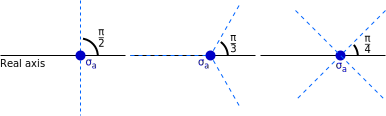
\includegraphics[width=12cm]{fig/asymptotes.pdf}
  \caption{The configuration of the asymptotes is always fixed given
    the number $N$ of asymptotes. Basically, the $N$ asympotes divide
    the complex plane into $N$ equal regions, and the angle from the
    real axis to the first asymptote is $\frac{\pi}{N}$.}
  \label{fig:asymptotes}
\end{figure}

Next, the intersection point of the asymptotes is given by
\[
\sigma_a = \frac{\sum \textrm{poles}-\sum \textrm{zeros}}{n_\textrm{poles} -
  n_\textrm{zeros}}.
\]

\begin{example}
  \label{ex:asymp}
  Consider the CE
  \[
  K(s+0.5) + (s^2+2s+5)(s^2+3s+20) = 0.
  \]
  There are four poles ($-1\pm 2j$, $-1.5\pm 4.2j$) and one zero
  ($-0.5$), therefore $4-1 = 3$ infinite branches. The asymptotes meet
  at
  \[
  \sigma_a = \frac{+0.5-1-1-1.5-1.5}{3} = -1.5.
  \]
  See Fig.~\ref{fig:rlocusasymp}.
  \begin{figure}[H]
    \centering
    \includegraphics[width=10cm]{fig/rlocusasymp.pdf}
    \caption{Root locus of $K(s+0.5) + (s+2s+5)(s^2+3s+20) = 0$, which
      has 1 finite and 3 infinite branches.}
    \label{fig:rlocusasymp}
  \end{figure}
\end{example}



\subsection{Poles/zeros on the real axis}

When there are poles/zeros on the real axis, then parts of the root
locus will be on the real axis. The rule is
\begin{quote}
  ``Every point of the real axis that is on the left of an odd number
  of poles/zeros belongs to the root locus.''
\end{quote}

From this rule, one can determine entirely the root locus on the real
axis, as well as the departure/arrival angles from/to the poles/zeros
on the real axis.

\begin{example}
  Fig.~\ref{fig:real} and~\ref{fig:real2} depict two typical
  configurations of poles/zeros on the real axis and how we can
  determine the root locus as well as departure/arrival angles on the
  real axis.
  \begin{figure}[H]
    \centering
    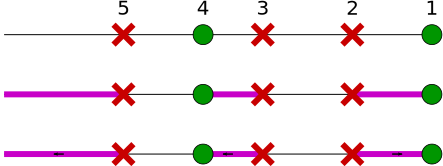
\includegraphics[width=7cm]{fig/real.pdf}
    \caption{A configuration of poles/zeros on the real axis. Red
      disks denote the poles and green squares the zeros. Step 1: we
      number the poles/zeros starting with 1 on the right. Step 2: we
      highlight the spaces between points 1 and 2, between points 3
      and 4, etc. as root locus. Step 3: we indicate the
      departure/arrival arrows (arrows must leave poles and arrive at
      zeros).}
    \label{fig:real}
  \end{figure}

  \begin{figure}[H]
    \centering
    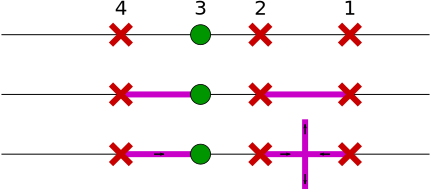
\includegraphics[width=7cm]{fig/real2.pdf}
    \caption{Another configuration. This configuration is the same as
      in Fig.~\ref{fig:real}, except that we have removed the
      rightmost zero. Doing so completely changes the root locus on
      the real axis. Note that, when determining the departure/arrival
      arrows, we have two arrows pointing towards each other between
      point 1 and point 2. This implies that there must exist a
      \emph{break-out} between point 1 and point 2. Similarly, in case
      we have two arrows pointing \emph{away} from each other, this
      will imply the existence of a \emph{break-in} point.}
    \label{fig:real2}
  \end{figure}
\end{example}


\subsection{Departure/arrival angles from/to complex poles/zeros}

It is important to determine the departure/arrival angles from
poles/zeros in order to have an accurate drawing of the root locus.

The angle of departure from a complex pole $p$ is given by
\[
\alpha_\textrm{dep}(p) = \pi - \sum_{\textrm{poles}\ p_i} \alpha_{p_i \to p} +
\sum_{\textrm{zeros}\ z_i} \alpha_{z_i \to p}.
\]

The angle $\alpha_{p_i \to p}$ can either be determined
graphically, or computed as $\angle (p-p_i)$. 

Note that, the angle of a complex number given in Cartesian form
$x+yj$ is \emph{not always} $\tan^{-1}(y/x)$ ! On modern calculators
or in Matlab/Python, it can be obtained as
\[
\angle (x+yj) = \mathrm{arctan2}(y,x).
\]

The angle of arrival to a complex pole $z$ is given by
\[
\alpha_\textrm{arr}(z) = \pi + \sum_{\textrm{poles}\ p_i} \alpha_{p_i \to z} -
\sum_{\textrm{zeros}\ z_i} \alpha_{z_i \to z}.
\]

\begin{example}
  Consider again the CE
  \[
  K(s+0.5) + (s^2+2s+5)(s^2+3s+20) = 0.
  \]
  We have seen in Example~\ref{ex:asymp} that this CE has four poles
  (let us number them from highest to lowers: $p_1=-1.5+4.2j,\ p_2=-1+
  2j,\ p_3=-1-2j,\ p_4=-1.5-4.2j$) and one zero ($z=-0.5$). Let us
  calculate the departure angle from one of the poles, say $p_2$. We
  have
  \begin{itemize}
  \item $\alpha_{p_1\to
      p_2}=\mathrm{arctan2}(2-4.2,-1+1.5)\simeq-1.35$\,rad;
      \item $\alpha_{p_3\to
      p_2}=\mathrm{arctan2}(2+2,-1+1)=\pi/2$\,rad;
  \item $\alpha_{p_4\to
      p_2}=\mathrm{arctan2}(2+4.2,-1+1.5)\simeq1.49$\,rad;
  \item $\alpha_{p_4\to
      p_2}=\mathrm{arctan2}(2-0,-1+0.5)\simeq1.82$\,rad.
  \end{itemize}
  Thus   
  \[
  \alpha_\textrm{dep}(p_2) \simeq \pi+1.35-\pi/2-1.49+1.82 \simeq
  3.24\,\mathrm{rad} \simeq 186\,\mathrm{degrees}.
  \]

  Fig.~\ref{fig:zoomedin} illustrates the above calculations.

  \begin{figure}[H]
    \centering
    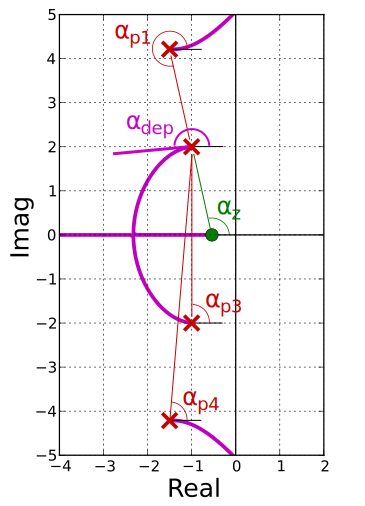
\includegraphics[width=7cm]{fig/zoomedin.pdf}
    \caption{Departure angle from a complex pole.}
    \label{fig:zoomedin}
  \end{figure}

\end{example}


\subsection{Break-in/break-out points}

Break-in/break-out points are points where two branches meet. It is
important to find these points to have an accurate drawing of the root
locus. Consider a break-in/break-out point $s$. Since two branches
meet at $s$, $s$ must be a \emph{double} root of the CE, which in turn
implies that $s$ cancels the CE \emph{and its derivative}, i.e.
\begin{equation}
  \label{eq:ppp}
  P(K,s) = 0\quad \textrm{and} \quad P'(K,s)=0.
\end{equation}
Since $P(K,s)=KN(s)+D(s)$, we have $P'(K,s)=KN'(s)+D'(s)$. From
(\ref{eq:ppp}), we have
\[
KN(s)+D(s)  \quad \textrm{and} \quad  KN'(s)+D'(s),
\]
i.e.
\[
\frac{D(s)}{N(s)} = -K = \frac{D'(s)}{N'(s)},
\]
which finally yields
\[
N'(s)D(s)-D'(s)N(s) = 0.
\]
Remark that the above equation is a polynomial equation which does not
contain $K$. It can then be solved to find $n$ roots,
$s_1$,\dots,$s_n$, which are candidates to be break-in/break-out
points. To verify whether any of these roots, say $s_i$, is indeed a
break-in/break-out point, we need to compute the corresponding $K$ by
\[
K = -\frac{D(s_i)}{N(s_i)},
\]
and verify that this $K$ is real positive. Example~\ref{ex:break}
illustrates the whole process through a numerical example.

\begin{example}
  \label{ex:break}
  Consider again the CE
  \[
  K(s+0.5) + (s^2+2s+5)(s^2+3s+20) = 0.
  \]
  Computing $N'(s)D(s)-D'(s)N(s)$ yields
  \[
  (s^4+5s^3+31s^2+55s+100)-(4s^3+15s^2+62s+55)(s+0.5)
  \]
  \[
  = -3s^4-12s^3-38.5s^2-31s+72.5.  
  \]
  The above polynomial has 4 roots, which are $s_{1,2}=-1.3\pm3.1j$,
  $s_3=-2.3$ and $s_4=0.9$. Substituting these values of $s$ into
  \[
  K = -\frac{(s^2+2s+5)(s^2+3s+20)}{s+0.5},
  \]
  we find out that $s_{1,2}$ correspond to $K=3.3\pm14.7j$, $s_3$
  to $K=58.1$ and $s_4$ to $K=-127.8$. Thus, there is only one
  break-in/break-out point at $s_3=-2.3$ and for
  $K=58.1$. Fig.~\ref{fig:rlocusasymp} confirms this result.
\end{example}



\subsection{Crossing of imaginary axis}

A point on the imaginary axis is given by $s=j\omega$. Pluging in
\[
KN(j\omega) + D(j\omega)=0.
\]
By separating the real and complex parts, one can find $K$ and
$\omega$.

This is important since it indicates when the system becomes unstable:
crossing the imaginary axis means that the root locus goes into the
RHP, which in turn means that the system becomes unstable.

\begin{example}
  \label{ex:crossing}
  Consider again the CE
  \[
  K(s+0.5) + (s^2+2s+5)(s^2+3s+20) = 0.
  \]
  Letting $s=j\omega$, one obtains
  \[
  K(j\omega+0.5) + [(j\omega)^2+2(j\omega)+5)][(j\omega)^2+3(j\omega)+20] = 0.
  \]
  \[
  j[-5\omega^3+(55+K)\omega] + [\omega^4-31\omega^2+100+0.5K] = 0.
  \]
  One thus have
  \[
  \left\{
  \begin{array}{lcr}
    -5\omega^3+(55+K)\omega &=& 0 \\
    \omega^4-31\omega^2+100+0.5K  &=& 0
  \end{array}
  \right.
  \]
  The first equation yields
  \begin{equation}
    \label{eq:KK}
    K = 5\omega^2-55.
  \end{equation}
  
  Substituting this expression of $K$ into the second equation yields
  \[
  \omega^4-28.5\omega^2+72.5=0,
  \]
  which has four solutions $\omega=\pm 1.68$ or $\omega=\pm 5.07$.
  
  From~(\ref{eq:KK}), we find that the solutions $\omega=\pm 1.68$
  correspond to $K=-40.9$ and the solutions $\omega=\pm 5.07$
  correspond to $K=73.4$. We can thus conclude that the root locus
  cross the imaginary axis for $\omega=\pm 5.07$ and $K=73.4$.
\end{example}

The gain $K$ where the system crosses the imaginary axis can also be
recovered by the Routh-Hurwitz criterion. 

\begin{example}
  Consider the same CE as in the previous example
  \[
  K(s+0.5) + (s^2+2s+5)(s^2+3s+20) = 0.
  \]
  Expanding this CE yields
  \[
  s^4+5s^3+31s^2+(55+K)s+(100+0.5K) = 0.
  \]
  Construct the Routh array

  \[
  \begin{array}{|c|c|c|c|}
    \hline
    s^4 & 1 & 31 &  100+0.5K\\
    \hline
    s^3 & 5 & 55+K &  \\
    \hline
    s^2 & \frac{100-K}{5} & 100+0.5K &\\
    \hline
    s & \frac{-K^2+32.5K+3000}{100-K}&0 & \\
    \hline
    1 & 100+0.5K& & \\
    \hline
  \end{array}
  \]
  
  The first column of the Routh array gives the following necessary
  and sufficient condition for stability: $K<100$ and
  $K^2-32.5K-3000<0$. The latter inequality yields
  $-40.9<K<73.4$. Therefore, the necessary and sufficient condition
  for stability is that $K<73.4$. We have thus recovered the result of
  Example~\ref{ex:crossing}.
\end{example}


\subsection{Summary}

\begin{summary}
  To sketch the root locus of a CE given in the form $KN(s) + D(s) = 0$,
  take the following steps
  \begin{enumerate}
  \item Compute the poles (roots of $D$) and the zeros (roots of $N$);
  \item Determine the number of infinite branches (=$n_\textrm{poles} -
    n_\textrm{zeros}$), which gives the number and configuration of the
    asymptotes. Compute the intersection point $\sigma_a$ of the
    asymptotes by
    \[
    \sigma_a = \frac{\sum \textrm{poles}-\sum \textrm{zeros}}{n_\textrm{poles} -
    n_\textrm{zeros}};
    \]
  \item Determine the locus on the real axis by considering the real
    poles and zeros;
  \item For each complex pole (resp. zero), compute the departure
    (resp. arrival) angle by
    \[
    \alpha_\textrm{dep}(p) = \pi - \sum_{\textrm{poles}\ p_i} \alpha_{p_i \to p} +
    \sum_{\textrm{zeros}\ z_i} \alpha_{z_i \to p}.
    \]
    \[
    \alpha_\textrm{arr}(z) = \pi + \sum_{\textrm{poles}\ p_i} \alpha_{p_i \to z} -
    \sum_{\textrm{zeros}\ z_i} \alpha_{z_i \to z}.
    \]
  \item Determine the break-in/break-out points by solving
    \[
    N'(s)D(s)-D'(s)N(s)=0;
    \]
  \item Determine the crossing of the imaginary axis by solving
    \[
    KN(j\omega) + D(j\omega)=0;
    \]
  \item Based on all the information obtained so far, sketch the root
    locus.
  \end{enumerate}
\end{summary}



\section{Transient response design by gain adjustment}
\label{sec:gainadj}

We have seen that the transient behavior depends on the locations of
the dominant (rightmost) poles : given performance specifications (in
terms of maximum overshoot, settling time, etc.), we can calculate the
desired damping coefficient $\zeta$ and undamped natural frequency
$\omega_n$, which in turn yield the desired locations for the dominant
pole(s) $s_\des$.

If $s_\des$ is on the root locus, then it means that gain adjustment
(i.e. varying $K$) alone is sufficient to set $s_\des$ as system
pole. To verify whether $s_\des$ is on the root locus, we can either
see graphically, or use the angle criterion as follows.

Assume that $s_\des$ is on the root locus. Then, there exists a $K$
such that $KN(s_\des)+D(s_\des)=0$, i.e. 
\[
\frac{D(s_\des)}{N(s_\des)} = -K,
\]
which implies
\[
\angle \frac{D(s_\des)}{N(s_\des)} = \angle (-K)  = \pi.
\]
Thus, if
\begin{equation}
  \label{eq:anglecrit}
\angle D(s_\des)-\angle N(s_\des) = \pi \mod 2\pi\footnote{``$\alpha = \beta
  \mod 2\pi$" means : there exists an integer $k$, such that $\alpha =
  \beta + 2k\pi$. For example, $\frac{pi}{4} = \frac{5\pi}{4}\mod 2\pi
  = \frac{5\pi}{4}\mod 2\pi$, etc.},  
\end{equation}
then the root locus goes through $s_\des$.

Next, \emph{if} the root locus indeed goes through $s_\des$, then one
can determine the corresponding gain $K$ by
\[
K = \frac{\|D(s_\des)\|}{\|N(s_\des)\|}.
\]

\begin{example}
  Consider the CE of the helicopter system with PD control
  [cf. Equation~\ref{eq:helicopd} in Section~\ref{eq:helicopd}], which
  can be rewritten as (for $m=2$, $k=0.5$)
  \[
  K[0.5(s+1)]+2s^2=0.
  \]
  Let us examine whether the root locus goes through $s_0=-2+j$ and
  $s_1=-1+j$, and if it does, determine the corresponding gain $K$.
  
  Applying the angle criterion for $s_0$ 
  \begin{eqnarray}
    \label{eq:toto}
    \angle D(s_0) - \angle N(s_0) &=&  \angle
    [2(-2+j)^2]  - \angle [0.5(-2+j+1)] \nonumber\\
    &=& \angle  [(-2+j)^2]  - \angle [(-2+j+1)] \nonumber\\
    &=& 2\angle(-2+j) - \angle (-1+j) \nonumber\\
    &=& 2[\pi-\mathrm{arctan}(0.5)]-\frac{3\pi}{4}\nonumber \\
    &\sim& 3.0 \neq \pi \mod 2\pi.\nonumber 
  \end{eqnarray}
  Thus, $s_0$ is \emph{not} on the root locus.

  Applying the angle criterion for $s_1$ 
  \begin{eqnarray}
    \label{eq:toto}
    \angle D(s_1) - \angle N(s_1) &=& \angle
    [(-1+j)^2] - \angle (-1+j+1)  \nonumber\\
    &=& 2\angle(-1+j) - \angle j = \frac{3\pi}{2} -  \frac{\pi}{2} = \pi\nonumber.
  \end{eqnarray}
  Thus, $s_1$ is on the root locus.

  Next, we can compute the gain $K$ that corresponds to $s_1$ by
  \[
  K = \frac{\|2(-1+j)^2\|}{\|0.5(-1+j+1)\|} = \frac{4}{0.5} = 8.
  \]
  One can verify these results graphically in
  Fig.~\ref{fig:rlocusex2}.
\end{example}

Finally, in case the system has zeros and/or is of order $>2$, we have
to make sure the second-order approximation is valid for the value of
$K$ just found. For this, we plug the value of $K$ into the CE,
evaluate the remaining poles, and verify that (see part I of the
course for more details)
\begin{itemize}
\item non-dominant poles are far to the left;
\item zeros are far to the left;
\item zeros that are not far to the left are cancelled by poles
  (pole/zero cancellation).
\end{itemize}

If necessary, we may simulate the response using Matlab/Python and
verify that the specifications are met.


\section{Improving transient behavior by lead compensation}

Section~\ref{sec:gainadj} addressed the case when the desired pole
location $s_\des$ is on the root locus. If this is not the case, then
one needs to \emph{reshape} the root locus and force it to go through
$s_\des$. There are two main ways to do so, either with a \emph{PD
  controller} or with a \emph{lead compensator} (in fact, PD
controllers can be seen as idealized versions of lead compensators).

\subsection{PD controller}
\label{sec:pddesign}

We have seen (e.g. in Fig.~\ref{fig:examplesystempd}) that a PD
controller can be represented as a block $(K_Ds+K_P)$ inserted before
the system to be controlled. This can be rewritten
\[
K_Ds+K_P = K_D\left(s+\frac{K_P}{K_D}\right) = K(s+z_c),
\]
where $K=K_D$ and $z_c=\frac{K_P}{K_D}$. Consider now a system with
and without PD control.

\begin{figure}[H]
  \label{fig:pddesign}
  \centering
  \tikzstyle{block} = [draw, fill=blue!20, rectangle, minimum height=3em, minimum width=4em]
  \tikzstyle{controller} = [draw, fill=red!20, rectangle, minimum height=3em, minimum width=4em]
  \tikzstyle{sum} = [draw, fill=blue!20, circle, node distance=1cm]
  \tikzstyle{input} = [coordinate]
  \tikzstyle{output} = [coordinate]
  \begin{tikzpicture}[auto, >=latex']
    % Nodes
    \node [input] (input) {};
    \node [sum, right = 0.5cm of input] (sum) {};
    \node [block, right = 0.5cm of sum] (system) {$K\frac{N}{D}$};
    \node [output, right = 1cm of system] (output) {};
    \node [input, below = 0.5cm of system] (m) {};
    % Arrows
    \draw [draw,->] (input) -- node {$R$} (sum);
    \draw [->] (sum) -- node {} (system);
    \draw [->] (system) -- node (y) {$C$}(output);
    \draw [-] (y) |- (m) {} ;
    \draw [->] (m) -| node[pos=0.99] {$-$}  node [near end] {} (sum);
  \end{tikzpicture}  
  \hspace{0.5cm}
  \begin{tikzpicture}[auto, >=latex']
    % Nodes
    \node [input] (input) {};
    \node [sum, right = 0.5cm of input] (sum) {};
    \node [controller, right = 0.5cm of sum] (system) {$K(s+z_c)$};
    \node [block, right = 0.5cm of system] (system2) {$\frac{N}{D}$};
    \node [output, right = 1cm of system2] (output) {};
    \node [input, below = 0.5cm of system] (m) {};
    % Arrows
    \draw [draw,->] (input) -- node {$R$} (sum);
    \draw [->] (sum) -- node {} (system);
    \draw [->] (system) -- (system2);
    \draw [->] (system2) -- node (y) {$C$}(output);
    \draw [-] (y) |- (m) {} ;
    \draw [->] (m) -| node[pos=0.99] {$-$}  node [near end] {} (sum);
  \end{tikzpicture}  
  \caption{Left: system without PD control. Right: system with PD control.}
\end{figure}

The CE for the system \emph{without PD} control is
\[
KN(s)+D(s) = 0.
\]
The fact that the root locus of this system does \emph{not} go through
$s_\des$ means that the angle criterion (\ref{eq:anglecrit}) is not
satisfied, i.e.
\[
\angle D(s_\des)-\angle N(s_\des) \neq \pi \mod 2\pi.
\]

The CE of the system \emph{with PD} control is
\[
K(s+z_c)N(s)+D(s) = 0.
\]
Since we want the root locus of the new system to go through $s_\des$,
we substitute $s_\des$ into the CE
\[
K(s_\des+z_c)N(s_\des)+D(s_\des) = 0.
\]
As the value of $s_\des$ is given, the above equation has only two
unknowns, $K$ and $z_c$. Examining the real and imaginary parts of the
equation yields two independent equations, which allows solving for
$K$ and $z_c$. Finally, the proportional and derivative gains are
finally given by
\[
K_D = K,\quad K_P = z_cK.
\]
Example~\ref{ex:pddesign} shows the method in action.

\begin{example}
  \label{ex:pddesign}
  Consider the system below. We would like to design a PD controller
  so that $s_\des=-2\pm1.9j$ are root of the system.

  \begin{figure}[H]
    \label{fig:pddesign}
    \centering
    \tikzstyle{block} = [draw, fill=blue!20, rectangle, minimum height=3em, minimum width=4em]
    \tikzstyle{controller} = [draw, fill=red!20, rectangle, minimum height=3em, minimum width=4em]
    \tikzstyle{sum} = [draw, fill=blue!20, circle, node distance=1cm]
    \tikzstyle{input} = [coordinate]
    \tikzstyle{output} = [coordinate]
    \begin{tikzpicture}[auto, >=latex']
      % Nodes
      \node [input] (input) {};
      \node [sum, right = 0.5cm of input] (sum) {};
      \node [block, right = 0.5cm of sum] (system) {$\frac{K}{(s+1)(s+2)(s+4)}$};
      \node [output, right = 1cm of system] (output) {};
      \node [input, below = 0.5cm of system] (m) {};
      % Arrows
      \draw [draw,->] (input) -- node {$R$} (sum);
      \draw [->] (sum) -- node {} (system);
      \draw [->] (system) -- node (y) {$C$}(output);
      \draw [-] (y) |- (m) {} ;
      \draw [->] (m) -| node[pos=0.99] {$-$}  node [near end] {} (sum);
    \end{tikzpicture}  
  \end{figure}

  The root locus of this system is given
  Fig.~\ref{fig:design-uncomp}.

  \begin{figure}[H]
    \centering
    \includegraphics[width=10cm]{fig/design-uncomp.pdf}
    \caption{Root locus of the uncompensated system.}
    \label{fig:design-uncomp}
  \end{figure}

  Clearly, the root locus does not go through $s_\des=-2\pm1.9j$.  To
  verify this, we apply the angle criterion
  \[
  \angle D(s_\des)-\angle N(s_\des)
  = \angle [(-2+1.9j+1)(-2+1.9j+2)(-2+1.9j+4)] 
  \]
  \[
  = \angle(-3.61-10.66j) \simeq 4.38\,\mathrm{rad}\neq \pi.
  \]
 
  We want now to find $K$ and $z_c$ such that
  \[
  K(s_\des+z_c)N(s_\des)+D(s_\des) = 0.  
  \]
  Substituting $s_\des=-2+1.9j$ yields
  \[
  K(-2+1.9j+z_c) + (-2+1.9j+1)(-2+1.9j+2)(-2+1.9j+4) =0, \quad \textrm{i.e.}
  \]
  \begin{equation}
    \label{eq:pdeq}
    [-3.61-(2-z_c)K] - [10.66-1.9K]j=0.  
  \end{equation}
  The imaginary part of~(\ref{eq:pdeq}) yields 
  \[
  K = \frac{10.66}{1.9} = 5.61.
  \]
  Substituting $K=5.61$ in the real part of~(\ref{eq:pdeq}) yields
  \[
  2-zc = \frac{-3.61}{5.61}=-0.64, \quad \textrm{i.e.} \quad z_c = 2+0.64 = 2.64.
  \]
  Finally,
  \[
  K_D = K = 5.61,\quad K_P= z_cK=14.83.
  \]

  The compensated system is thus given by

  \begin{figure}[H]
    \centering
    \tikzstyle{block} = [draw, fill=blue!20, rectangle, minimum height=3em, minimum width=4em]
    \tikzstyle{controller} = [draw, fill=red!20, rectangle, minimum height=3em, minimum width=4em]
    \tikzstyle{sum} = [draw, fill=blue!20, circle, node distance=1cm]
    \tikzstyle{input} = [coordinate]
    \tikzstyle{output} = [coordinate]
    \begin{tikzpicture}[auto, >=latex']
      % Nodes
      \node [input] (input) {};
      \node [sum, right = 0.5cm of input] (sum) {};
      \node [controller, right = 0.5cm of sum] (system) {$K(s+2.64)$};
      %\node [controller, right = 0.5cm of sum] (system) {$K(s+z_c)$};
      \node [block, right = 0.5cm of system] (system2) {$\frac{1}{(s+1)(s+2)(s+4)}$};
      \node [output, right = 1cm of system2] (output) {};
      \node [input, below = 0.5cm of system] (m) {};
      % Arrows
      \draw [draw,->] (input) -- node {$R$} (sum);
      \draw [->] (sum) -- node {} (system);
      \draw [->] (system) -- (system2);
      \draw [->] (system2) -- node (y) {$C$}(output);
      \draw [-] (y) |- (m) {} ;
      \draw [->] (m) -| node[pos=0.99] {$-$}  node [near end] {} (sum);
    \end{tikzpicture}  
  \end{figure}

  The root locus of the compensated system is given in
  Fig.~\ref{fig:design-PD}. We can see that the root locus indeed goes
  through $s_\des=-2\pm1.9j$ for $K=5.61$.

  \begin{figure}[H]
    \centering
    \includegraphics[width=10cm]{fig/design-PD.pdf}
    \caption{System compensated with PD controller.}
    \label{fig:design-PD}
  \end{figure}


\end{example}

\subsection{Lead compensator}
\label{sec:lead}

We have seen that PD controllers were able to force the root locus to
go through almost arbitrary desired root locations. However, there are
two main drawbacks with PD controllers
\begin{itemize}
\item PD controllers cannot be realized via \emph{passive} circuits
  (mass-spring-dampers for mechanical systems,
  resistor-inductor-capacitor for electronic circuits): additional
  power must be provided by \emph{active} components, such as
  operational amplifiers;
\item PD controllers are sensitive to noise (see below).
\end{itemize}

One way to address these drawbacks consists in using \emph{lead
  compensators}. A lead compensator is a block with transfer function
$K\frac{s+z_c}{s+p_c}$ that is inserted before the system to be
controlled. We can see that a lead compensator is similar to a PD
controller, except for the term $1/(s+p_c)$.

\begin{figure}[H]
  \label{fig:pddesign}
  \centering
  \tikzstyle{block} = [draw, fill=blue!20, rectangle, minimum height=3em, minimum width=4em]
  \tikzstyle{controller} = [draw, fill=red!20, rectangle, minimum height=3em, minimum width=4em]
  \tikzstyle{sum} = [draw, fill=blue!20, circle, node distance=1cm]
  \tikzstyle{input} = [coordinate]
  \tikzstyle{output} = [coordinate]
  \begin{tikzpicture}[auto, >=latex']
    % Nodes
    \node [input] (input) {};
    \node [sum, right = 0.5cm of input] (sum) {};
    \node [controller, right = 0.5cm of sum] (system) {$K\frac{s+z_c}{s+p_c}$};
    \node [block, right = 0.5cm of system] (system2) {$\frac{N}{D}$};
    %\node [block, right = 0.5cm of system] (system2) {$\frac{1}{(s+1)(s+2)(s+4)}$};
    \node [output, right = 1cm of system2] (output) {};
    \node [input, below = 0.5cm of system] (m) {};
    % Arrows
    \draw [draw,->] (input) -- node {$R$} (sum);
    \draw [->] (sum) -- node {} (system);
    \draw [->] (system) -- (system2);
    \draw [->] (system2) -- node (y) {$C$}(output);
    \draw [-] (y) |- (m) {} ;
    \draw [->] (m) -| node[pos=0.99] {$-$}  node [near end] {} (sum);
  \end{tikzpicture}  
  \caption{System with lead compensator.}
\end{figure}


% \begin{figure}[H]
%   \label{fig:pddesign}
%   \centering
%   \tikzstyle{block} = [draw, fill=blue!20, rectangle, minimum height=3em, minimum width=4em]
%   \tikzstyle{controller} = [draw, fill=red!20, rectangle, minimum height=3em, minimum width=4em]
%   \tikzstyle{sum} = [draw, fill=blue!20, circle, node distance=1cm]
%   \tikzstyle{input} = [coordinate]
%   \tikzstyle{output} = [coordinate]
%   \begin{tikzpicture}[auto, >=latex']
%     % Nodes
%     \node [input] (input) {};
%     \node [sum, right = 0.5cm of input] (sum) {};
%     \node [controller, right = 0.5cm of sum] (system) {$K\frac{s+0.2}{s+0.05}$};
%     \node [block, right = 0.5cm of system] (system2) {$\frac{1}{s(s+3)(s+4)}$};
%     \node [output, right = 1cm of system2] (output) {};
%     \node [input, below = 0.5cm of system] (m) {};
%     % Arrows
%     \draw [draw,->] (input) -- node {$R$} (sum);
%     \draw [->] (sum) -- node {} (system);
%     \draw [->] (system) -- (system2);
%     \draw [->] (system2) -- node (y) {$C$}(output);
%     \draw [-] (y) |- (m) {} ;
%     \draw [->] (m) -| node[pos=0.99] {$-$}  node [near end] {} (sum);
%   \end{tikzpicture}  
%   \begin{tikzpicture}[auto, >=latex']
%     % Nodes
%     \node [input] (input) {};
%     \node [sum, right = 0.5cm of input] (sum) {};
%     \node [controller, right = 0.5cm of sum] (system) {$K\frac{s+0.1}{s}$};
%     \node [block, right = 0.5cm of system] (system2) {$\frac{1}{s(s+3)(s+4)}$};
%     \node [output, right = 1cm of system2] (output) {};
%     \node [input, below = 0.5cm of system] (m) {};
%     % Arrows
%     \draw [draw,->] (input) -- node {$R$} (sum);
%     \draw [->] (sum) -- node {} (system);
%     \draw [->] (system) -- (system2);
%     \draw [->] (system2) -- node (y) {$C$}(output);
%     \draw [-] (y) |- (m) {} ;
%     \draw [->] (m) -| node[pos=0.99] {$-$}  node [near end] {} (sum);
%   \end{tikzpicture}  
%   \caption{System with lead compensator.}
% \end{figure}


% Applying the angle criterion as in Section~\ref{sec:pddesign}, we
% find that $z_c$ and $p_c$ must obey
% \begin{equation}
%   \label{eq:lead}
%   \angle(s_\des+z_c)-\angle(s_\des+p_c) = \alpha_\mathrm{def} \mod 2\pi,
% \end{equation}

% where $\alpha_\mathrm{def}$ is the angle deficiency given, as
% previously, by
% \[
% \alpha_\mathrm{def}= \angle D(s_\des)-\angle N(s_\des) - \pi.
% \]

The CE of the system with lead compensator becomes
\[
K(s+z_c)N(s) + (s+p_c)D(s)=0.
\]
Since we want the root locus of the new system to go through $s_\des$,
we substitute $s_\des$ into the CE
\begin{equation}
  \label{eq:lead}
  K(s_\des+z_c)N(s_\des)+(s_\des+p_c)D(s_\des) = 0.  
\end{equation}

As the value of $s_\des$ is given, the above equation has three
unknowns, $K$, $z_c$ and $p_c$. Examining the real and imaginary parts
of the equation yields two independent equations. Two equations and
three unknowns means that, contrary to the PD controller case, there
are \emph{multiple} values of $K$, $z_c$ and $p_c$ that can satisfy
(\ref{eq:lead}). However, if we fix a particular value for $z_c$, then
$K$ and $p_c$ will be uniquely determined. In practice, we shall
choose a sensible value for $z_c$, and then determine the
corresponding values for $K$ and $p_c$, as shown in
Example~\ref{ex:lead}.

\begin{example}
  \label{ex:lead}
  Consider the same system as in Example~\ref{ex:pddesign}. We shall
  design a lead compensator so that $s_\des = 2\pm 1.9j$ are roots of
  the system.

  First of all, we compute the $z^*_c$ that corresponds to the PD
  controller. We saw in Example~\ref{ex:pddesign} that the this value
  is $z^*_c=2.64$. The possible (and desirable) values for $z_c$ will
  be smaller than that critical value, yielding less derivation.

  As stated in the main text, there are multiple possible values for
  $z_c$: in fact, any $z_c$ verifying $0<z_c<z^*_c$ is possible. Let
  fix $z_c=1.5$ and study how we can compute the
  corresponding $p_c$.

  Substituting $s_\des=-2+1.9j$ and $z_c=1.5$ in~(\ref{eq:lead})
  yields
  \[
  K(-2+1.9j+1.5) +
  \]
  \[
  (-2+1.9j+p_c)(-2+1.9j+1)(-2+1.9j+2)(-2+1.9j+4) =0, \quad \textrm{i.e.}
  \]
  \begin{equation}
    \label{eq:leadeq}
    [27.47-3.61p_c-0.5K] - [14.46-10.66p_c+1.9K]j=0.  
  \end{equation}
  We thus have the following $2\times 2$ linear system
  \[
  \left\{
    \begin{array}{ccc}
      -3.61p_c-0.5K&=&-27.47\\
      -10.66p_c+1.9K&=&-14.46
    \end{array}
  \right.,
  \]
  which yields the solution $p_c=4.88$, $K=19.74$.

  As stated in the main text, different values of $z_c$ will yield
  different values of $p_c$ and $K$. For example,
  \begin{itemize}
  \item If $z_c=1$, we shall find $p_c=3.80$ and $K=13.74$;
  \item If $z_c=0.5$, we shall find $p_c=3.23$ and $K=10.53$.
  \end{itemize}

  The following figures plot the root locus for the three cases.

  \begin{figure}[H]
    \centering
    \includegraphics[width=8cm]{fig/design-lead15.pdf}
    \caption{System with lead compensation $\frac{s+1.5}{s+4.88}$.}
    \label{fig:design-lead15}
  \end{figure}
  \begin{figure}[H]
    \centering
    \includegraphics[width=8cm]{fig/design-lead10.pdf}
    \caption{System with lead compensation $\frac{s+1}{s+3.80}$.}
    \label{fig:design-lead10}
  \end{figure}

  \begin{figure}[H]
    \centering
    \includegraphics[width=8cm]{fig/design-lead05.pdf}
    \caption{System with lead compensation $\frac{s+0.5}{s+3.23}$.}
    \label{fig:design-lead05}
  \end{figure}

  Let us now compare the steady-state errors to unit step input of the
  different compensated sytems (which are all of type 0).

  Recall first that the position constant\,\footnote{Note that the
    position constant $K_p$ and the proportional gain $K_P$ are two
    different objects.} is given by
  \[
  K_p = \lim_{s\to 0} K(s+z_c)\frac{N(s)}{D(s)} = \frac{Kz_c}{8}
  \]
  and
  \[
  K_p = \lim_{s\to 0} K\frac{s+z_c}{s+p_c}\frac{N(s)}{D(s)} = \frac{Kz_c}{8p_c}
  \]
  for the PD controller and the lead compensators respectively. The
  steady-state error for unit step input is then given by
  \[
  e_\sse = \frac{1}{1+K_p}.
  \]

  \vspace{0.2cm}

  \begin{tabular}{|c|c|c|c|c|}
    \hline
    &PD control&Lead comp 1&Lead comp 2&Lead comp 3\\\hline
    $z_c$&2.64&1.5&1&0.5\\\hline      
    $p_c$&NA&4.88&3.80&3.23\\\hline      
    $K$&5.61&19.74&13.74&10.53\\\hline      
    $K_p$&1.85&0.76&0.45&0.20\\\hline      
    $e_\sse$&0.35&0.57&0.69&0.83\\\hline      
  \end{tabular}

  \vspace{0.2cm}

  We can observe that the PD controller yields the best steady-state
  behavior, and that steady-state performance of the lead compensators
  decreases as $z_c$ becomes smaller, i.e. as they grow further away
  from the PD controller, their ideal representative.

  The choice of the appropriate lead compensator in a particular
  application will ultimately depend on a trade-off among many
  factors, including
  \begin{itemize}
  \item goodness of second-order approximation;
  \item desired steady-state error;
  \item sensitivity to noise;
  \item ease of implementation with physical components,\dots
  \end{itemize}
\end{example}

Let us now explain why lead compensators are less sensitive to noise
than PD controllers. Basically, noise is a signal with very high
frequency. We shall see in Chapter~\ref{chap:fr} that the amplitude of
the response of a system with transfer function $G$ to a signal of
frequency $\omega$ is given by $\|G(j\omega)\|$. Thus, the amplitude
of the response of a PD controller is $\|K(j\omega+z_c)\|$, which
converges to $\infty$ ans $\omega\to\infty$. On the other hand, the
amplitude of the response of a lag compensator is
\[
\frac{K\|j\omega+z_c\|}{\|j\omega+p_c\|},
\]
which converges to $K$ as $\omega\to\infty$.


\section{Reducing steady-state error by lag compensation}

Suppose that the original system has a good transient behavior, but
its steady-state error does not meet the specifications. The idea here
thus consists in improving the steady-state error \emph{without}
changing noticeably the root locus, thereby preserving the transient
behavior. There are two main ways to do so, either with a \emph{PI
  controller} or with a \emph{lag compensator} (in fact, PI
controllers can be seen as idealized versions of lag compensators).

\subsection{PI controller}

A PI controller can be represented as a block $(K_P+\frac{K_I}{s})$
inserted before the system to be controlled. This can be rewritten as
\[
K_P+\frac{K_I}{s} = \frac{K_Ps+K_I}{s} =
\frac{K_P\left(s+\frac{K_I}{K_P}\right)}{s} = \frac{K(s+z_c)}{s}
\]
where $K=K_P$ and $z_c=\frac{K_I}{K_P}$. Consider now a type-1 system
with and without PI control.

\begin{figure}[H]
  \label{fig:pddesign}
  \centering
  \tikzstyle{block} = [draw, fill=blue!20, rectangle, minimum height=3em, minimum width=4em]
  \tikzstyle{controller} = [draw, fill=red!20, rectangle, minimum height=3em, minimum width=4em]
  \tikzstyle{sum} = [draw, fill=blue!20, circle, node distance=1cm]
  \tikzstyle{input} = [coordinate]
  \tikzstyle{output} = [coordinate]
  \begin{tikzpicture}[auto, >=latex']
    % Nodes
    \node [input] (input) {};
    \node [sum, right = 0.5cm of input] (sum) {};
    \node [block, right = 0.5cm of sum] (system) {$\frac{KN}{sD}$};
    \node [output, right = 1cm of system] (output) {};
    \node [input, below = 0.5cm of system] (m) {};
    % Arrows
    \draw [draw,->] (input) -- node {$R$} (sum);
    \draw [->] (sum) -- node {} (system);
    \draw [->] (system) -- node (y) {$C$}(output);
    \draw [-] (y) |- (m) {} ;
    \draw [->] (m) -| node[pos=0.99] {$-$}  node [near end] {} (sum);
  \end{tikzpicture}  
  \hspace{0.5cm}
  \begin{tikzpicture}[auto, >=latex']
    % Nodes
    \node [input] (input) {};
    \node [sum, right = 0.5cm of input] (sum) {};
    \node [controller, right = 0.5cm of sum] (system) {$K\frac{s+z_c}{s}$};
    \node [block, right = 0.5cm of system] (system2) {$\frac{N}{sD}$};
    \node [output, right = 1cm of system2] (output) {};
    \node [input, below = 0.5cm of system] (m) {};
    % Arrows
    \draw [draw,->] (input) -- node {$R$} (sum);
    \draw [->] (sum) -- node {} (system);
    \draw [->] (system) -- (system2);
    \draw [->] (system2) -- node (y) {$C$}(output);
    \draw [-] (y) |- (m) {} ;
    \draw [->] (m) -| node[pos=0.99] {$-$}  node [near end] {} (sum);
  \end{tikzpicture}  
  \caption{Left: type-1 system without PI control (note that $N$ and
    $D$ must contain no ``$s$'' term for the system to be of
    type~1). Right: the same system with PI control.}
\end{figure}

Since the original system is of type 1, it has 0 steady-state error to
step input. For ramp input, let us compute the \emph{velocity constant}
\[
K_v = \lim_{s\to 0} sK\frac{N(s)}{sD(s)} = \frac{KN(0)}{D(0)}.
\]
Note that $N(0)\neq0$ and $D(0)\neq0$ since $N$ and $D$ do not contain
any ``$s$'' term.

Next, the steady-state error to ramp input is given by
\begin{equation}
  \label{eq:ess-uncomp}
  e_\sse = \frac{1}{K_v} = \frac{D(0)}{KN(0)} \neq 0.
\end{equation}

For the system with PI control, we have
\[
K_v = \lim_{s\to 0} sK\frac{s+z_c}{s}\frac{N(s)}{sD(s)} = \lim_{s\to 0}
\frac{KN(0)}{sD(0)} = \infty.
\]

Thus, the steady-state error to ramp input of the system with PI
control is given by
\[
e_\sse = \frac{1}{K_v} = 0.
\]

Thus, PI control enables cancelling the steady state error to ramp
inputs for type-1 systems. A similar reasoning applies to step inputs
and type-0 systems, parabolic inputs and type-2 systems, etc.

In fact, as can be seen directly from the block diagram, the PI
controller increases the type of a given system by 1 (type-0 systems
become type-1, type-1 systems become type-2, etc.)

Let us now examine how the PI controller affects the transient
behavior. Adding the PI controller amounts to adding a new pole at
$s=0$ and a new zero at $s=-z_c$. Thus, if $z_c$ is very small, then
the new pole and new zero will \emph{cancel} each other, leaving the
root locus, hence the transient behavior, almost unchanged.

\begin{example}
  \label{ex:pidesign}
  Consider the system below. We would like to design a PI controller
  that eliminates steady-state error to ramp inputs without changing
  the transient behavior.
  \begin{figure}[H]
    \label{fig:pddesign}
    \centering
    \tikzstyle{block} = [draw, fill=blue!20, rectangle, minimum height=3em, minimum width=4em]
    \tikzstyle{controller} = [draw, fill=red!20, rectangle, minimum height=3em, minimum width=4em]
    \tikzstyle{sum} = [draw, fill=blue!20, circle, node distance=1cm]
    \tikzstyle{input} = [coordinate]
    \tikzstyle{output} = [coordinate]
    \begin{tikzpicture}[auto, >=latex']
      % Nodes
      \node [input] (input) {};
      \node [sum, right = 0.5cm of input] (sum) {};
      \node [block, right = 0.5cm of sum] (system) {$\frac{K}{s(s+3)(s+4)}$};
      \node [output, right = 1cm of system] (output) {};
      \node [input, below = 0.5cm of system] (m) {};
      % Arrows
      \draw [draw,->] (input) -- node {$R$} (sum);
      \draw [->] (sum) -- node {} (system);
      \draw [->] (system) -- node (y) {$C$}(output);
      \draw [-] (y) |- (m) {} ;
      \draw [->] (m) -| node[pos=0.99] {$-$}  node [near end] {} (sum);
    \end{tikzpicture}  
  \end{figure}

  First, we sketch the root locus of this system in
  Fig.~\ref{fig:design-uncomp2}.

  \begin{figure}[H]
    \centering
    \includegraphics[width=10cm]{fig/design-uncomp2.pdf}
    \caption{Root locus of the uncompensated system.}
    \label{fig:design-uncomp2}
  \end{figure}

  Assume that the desired transient behavior of this system
  corresponds the roots $s_\des=-0.76\pm 1.75j$ and achieved for
  $K=20$.

  Next, the velocity constant and the steady-state error to unit ramp
  intput are given by 
  \[
  K_v =  \lim_{s\to 0} sK\frac{1}{s(s+3)(s+4)} = \frac{20}{12} = \frac{5}{3},
  \]
  \[
  e_\sse = \frac{1}{K_v} = \frac{3}{5} = 0.6.
  \]

  Consider now two PI controllers with $z_c=0.2$ and $z_c=0.1$. The
  root loci of the two compensated systems are given in
  Fig.~\ref{fig:design-PI} and Fig.~\ref{fig:design-PI2}.

  \begin{figure}[H]
    \centering
    \includegraphics[width=10cm]{fig/design-PI.pdf}
    \caption{System compensated with PI controller ($z_c=0.2$).}
    \label{fig:design-PI}
  \end{figure}

  \begin{figure}[H]
    \centering
    \includegraphics[width=10cm]{fig/design-PI2.pdf}
    \caption{System compensated with PI controller ($z_c=0.1$).}
    \label{fig:design-PI2}
  \end{figure}

  From the theoretical analysis in the main text, the steady-state
  error to ramp inputs becomes 0. At the same time, we can observe
  that the root locus changes a bit for $z_c=0.2$ and very little for
  $z_c=0.1$. In fact, for $z_c\to 0$, the root locus will become
  identical to that of the original system. 
  
  In particular, the poles of the PI-controlled system for $K=20$ are
  given by 
  \begin{itemize}
  \item $\{-5.45,-0.66\pm1.67j,-0.23\}$ for $z_c=0.2$;
  \item $\{-5.46,-0.72\pm1.71j,-0.11\}$ for $z_c=0.1$.
  \end{itemize}

  Thus, as $z_c$ becomes smaller, the dominant pole will get closer to
  $z_c$, yielding a better pole/zero compensation, while the two
  complex poles with get closer to $s_\des=-0.76\pm1.75j$.

  To illustrate the above development, we plot the response of the
  original system and the compensated systems to unit step and ramp
  inputs in Fig.~\ref{fig:design-PI-resp}. We can see that the step
  response of the compensated systems are similar to the original
  system while the ramp error is reduced from 0.6 in the original
  system to 0 in the compensated systems.

  \begin{figure}[H]
    \centering
    \includegraphics[width=5.5cm]{fig/design-PI-resp.pdf}
    \includegraphics[width=5.5cm]{fig/design-PI-resp2.pdf}
    \caption{Left: response to unit step. Right: error to unit ramp.}
    \label{fig:design-PI-resp}
  \end{figure}

\end{example}


\subsection{Lag compensator}
\label{sec:lag}

PI controllers, as PD controllers, cannot be realized by passive
components. Thus, similarly to lead compensators, which approximate PD
controllers, we introduce here lag compensators, which approximate PI
controllers, but which can be realized by passive components.

Recall that PI controllers are basically a block with transfer
function $K\frac{s+z_c}{s}$ where $z_c$ is very small. Lag
compensators are given by the transfer function $K\frac{s+z_c}{s+p_c}$
where $z_c$ and $p_c$ are very small, and $p_c$ is very small compared
to $z_c$. Consider the same type-1 system as previously, now with a
lag compensator.

\begin{figure}[H]
  \label{fig:pddesign}
  \centering
  \tikzstyle{block} = [draw, fill=blue!20, rectangle, minimum height=3em, minimum width=4em]
  \tikzstyle{controller} = [draw, fill=red!20, rectangle, minimum height=3em, minimum width=4em]
  \tikzstyle{sum} = [draw, fill=blue!20, circle, node distance=1cm]
  \tikzstyle{input} = [coordinate]
  \tikzstyle{output} = [coordinate]
  \begin{tikzpicture}[auto, >=latex']
    % Nodes
    \node [input] (input) {};
    \node [sum, right = 0.5cm of input] (sum) {};
    \node [controller, right = 0.5cm of sum] (system) {$K\frac{s+z_c}{s+p_c}$};
    \node [block, right = 0.5cm of system] (system2) {$\frac{N}{sD}$};
    \node [output, right = 1cm of system2] (output) {};
    \node [input, below = 0.5cm of system] (m) {};
    % Arrows
    \draw [draw,->] (input) -- node {$R$} (sum);
    \draw [->] (sum) -- node {} (system);
    \draw [->] (system) -- (system2);
    \draw [->] (system2) -- node (y) {$C$}(output);
    \draw [-] (y) |- (m) {} ;
    \draw [->] (m) -| node[pos=0.99] {$-$}  node [near end] {} (sum);
  \end{tikzpicture}  
  \caption{Type-1 system with lag compensation.}
\end{figure}

Compute again the velocity constant and the steady-state error to unit
ramp input for the compensated system
\[
K_v = \lim_{s\to 0} sK\frac{s+z_c}{s+p_c}\frac{N(s)}{sD(s)} = \lim_{s\to 0}
\frac{KN(0)}{D(0)}\frac{z_c}{p_c},
\]
\[
e_\sse = \frac{1}{K_v} = \frac{D(0)}{KN(0)}\frac{p_c}{z_c}.
\]

Thus, the steady-state error has been reduced by a factor
$\frac{p_c}{z_c}$ as compared to the uncompensated
system~(\ref{eq:ess-uncomp}). Thus, if $p_c\ll z_c$, then the
steady-state error can become very small.

Regarding the transient behavior, if both $p_c$ and $z_c$ are very
close to zero, then we shall have pole/zero cancellation. Thus, the
root locus of the system will be changed very little.

\begin{example}
  \label{ex:lag}
  Consider the same system as in Example~\ref{ex:pddesign}. We would
  like to design a lag compensator to reduce the steady-state error by
  a factor 4 without changing noticeably the transient behavior.

  We choose $p_c=0.05$ and $z_c=0.2$ so that
  $\frac{p_c}{z_c}=\frac{1}{4}$ and $p_c$ and $z_c$ are small
  enough. The root locus is given in Fig.~\ref{fig:design-lag} and
  Fig.~\ref{fig:design-lag-zoom}. We can observe that the root locus
  has been changed a little.

  \begin{figure}[H]
    \centering
    \includegraphics[width=10cm]{fig/design-lag.pdf}
    \caption{Root locus of the system with lag compensation.}
    \label{fig:design-lag}
  \end{figure}

  \begin{figure}[H]
    \centering
    \includegraphics[width=10cm]{fig/design-lag-zoom.pdf}
    \caption{Zoomed in near 0.}
    \label{fig:design-lag-zoom}
  \end{figure}

  Note that we could also choose $p_c=0.005$ and $z_c=0.02$, which
  would give us the same reduction in terms of steady-state error but
  which would yield a root locus even closer to the original
  one. In fact, there are infinitely many ways to choose these
  values. Ultimately, the choice of the appropriate lag compensator in a
  particular application will ultimately depend on a trade-off among
  many factors, including
  \begin{itemize}
  \item stability of the compensated system;
  \item desired steady-state error;
  \item closeness to original root locus;
  \item ease of implementation with physical components,\dots
  \end{itemize}

\end{example}


\section{Improving transient behavior \emph{and} reducing steady-state
  error}

To improve both transient behavior \emph{and} reducing steady-state
error, we can combine PD and PI controllers into a PID controller
(ideal case) or we can combine lead and lag compensators into a
lead-lag compensator (realizable with passive components).


\subsection{PID controller}

Consider a system with feedforward transfer function $G(s)$. We first
design a PD controller $K_1(s+z_{c1})$ to meet the transients
specifications. Then, we design a PI controller
$K_2\frac{s+z_{c2}}{s}$ for the system with feedforward TF
$K_1(s+z_{c1})G(s)$ to meet the steady-state specifications without
noticeably changing the transient behavior achieved previously. The
resulting system will have a feedforward TF given by
\[
K_2\frac{s+z_{c2}}{s}K_1(s+z_{c1})G(s).
\]

The TF of the PID controller can also be rewritten as
\[
 K_1K_2\left(s+(z_{c1}+z_{c2})+\frac{z_{c1}z_{c2}}{s}\right)
= K_D s  + K_P + \frac{K_I}{s},
\]
where $K_D=K_1K_2$, $K_P=K_1K_2(z_{c1}+z_{c2})$, and
$K_I=K_1K_2z_{c1}z_{c2}$.

\subsection{Lead-lag compensator}

Here, we first design a lead compensator
$K_1\frac{s+z_{c1}}{s+p_{c1}}$, with $p_{c1}>z_{c_1}$, to meet the
transients specifications. Then, we design a lag compensator
$K_2\frac{s+z_{c2}}{s+p_{c2}}$, with $p_{c1}<z_{c_1}\ll 1$, for the
lead-compensated system to meet the steady-state specifications
without noticeably changing the transient behavior achieved
previously. The resulting system will have a feedforward TF given by
\[
K_2\frac{s+z_{c2}}{s+p_{c2}}K_1\frac{s+z_{c1}}{s+p_{c1}}G(s) =
K_1K_2\frac{(s+z_{c1})(s+z_{c2})}{(s+p_{c1})(s+p_{c2})} G(s).
\]
Furthermore, if $\frac{z_{c1}}{p_{c1}}=\frac{p_{c2}}{z_{c2}}$, the TF
of the lead-lag compensator can be rewritten as
\[
K\frac{(s+\frac{1}{T_1})(s+\frac{1}{T_2})}{(s+\frac{1}{\alpha
    T_1})(s+\frac{\alpha}{T_2})},
\]
where $K=K_1K_2$, $T_1=\frac{1}{z_{c1}}$, $T_2=\frac{1}{z_{c2}}$,
$\alpha=\frac{z_{c1}}{p_{c1}}=\frac{p_{c2}}{z_{c2}}>1$.


\section{Physical implementation of compensators}


\subsection{Lead compensators}

Consider the electrical circuit in Fig.~\ref{fig:impl-lead}. Its
transfer function is given by
\[
\frac{V_o}{V_i} = \frac{s+\frac{1}{R_1C}}{s+\frac{1}{R_1C}+\frac{1}{R_2C}}.
\]

\begin{figure}[H]
  \centering
  \includegraphics[width=5cm]{fig/impl-lead.pdf}
  \caption{Electrical implementation of a lead compensator.}
  \label{fig:impl-lead}
\end{figure}

Thus, given desired $z_c$ and $p_c$, we can choose $R_1$, $R_2$ and
$C$ such that
\[
R_1C = \frac{1}{z_c},\quad R_2C = \frac{1}{p_c-z_c}.
\]

Note that the amplification gain $K$ still needs to be realized by
an active element.


\subsection{Lag compensators}

Consider the electrical circuit in Fig.~\ref{fig:impl-lag}. Its
transfer function is given by
\[
\frac{V_o}{V_i} = \frac{R_2}{R_1+R_2}\frac{s+\frac{1}{R_2C}}{s+\frac{1}{(R_1+R_2)C}}.
\]

\begin{figure}[H]
  \centering
  \includegraphics[width=4cm]{fig/impl-lag.pdf}
  \caption{Electrical implementation of a lag compensator.}
  \label{fig:impl-lag}
\end{figure}

Thus, given desired $z_c$ and $p_c$, we can choose $R_1$, $R_2$ and
$C$ such that
\[
R_1C = \frac{1}{z_c},\quad R_2C = \frac{1}{p_c}-\frac{1}{z_c}.
\]

Note that the amplification gain $K$ still needs to be realized by
an active element.


\section{Parallel compensation}

Up to now, we have considered \emph{series} controllers/compensators,
which are inserted in series before the system. It is also possible to
perform \emph{parallel} compensation by placing a new element in a
\emph{minor feedback loop} in parallel with the system.

Consider the same generic unit feedback system as in
Fig.~\ref{fig:pddesign} but now with parallel compensation.

\begin{figure}[H]
  \label{fig:parallel}
  \centering
  \tikzstyle{block} = [draw, fill=blue!20, rectangle, minimum height=3em, minimum width=4em]
  \tikzstyle{controller} = [draw, fill=red!20, rectangle, minimum height=1.5em, minimum width=4em]
  \tikzstyle{sum} = [draw, fill=blue!20, circle, node distance=1cm]
  \tikzstyle{input} = [coordinate]
  \tikzstyle{output} = [coordinate]
  \adjustbox{valign=t}{
    \begin{tikzpicture}[auto, >=latex']
      % Nodes
      \node [input] (input) {};
      \node [sum, right = 0.5cm of input] (sum) {};
      \node [block, right = 0.5cm of sum] (system) {$K\frac{N}{D}$};
      \node [output, right = 1cm of system] (output) {};
      \node [input, below = 0.5cm of system] (m) {};
      % Arrows
      \draw [draw,->] (input) -- node {$R$} (sum);
      \draw [->] (sum) -- node {} (system);
      \draw [->] (system) -- node (y) {$C$}(output);
      \draw [-] (y) |- (m) {} ;
      \draw [->] (m) -| node[pos=0.99] {$-$}  node [near end] {} (sum);
    \end{tikzpicture}}
  \hspace{0.5cm}
  \adjustbox{valign=t}{
    \begin{tikzpicture}[auto, >=latex']
      % Nodes
      \node [input] (input) {};
      \node [sum, right = 0.5cm of input] (sum) {};
      \node [sum, right = 0.5cm of sum] (sum2) {};
      \node [block, right = 0.5cm of sum2] (system) {$K\frac{N}{D}$};
      \node [output, right = 1.5cm of system] (output) {};
      \node [controller, below = 0.2cm of system] (gc) {$G_c$};
      \node [input, below = 1cm of system] (m) {};
      % Arrows
      \draw [draw,->] (input) -- node {$R$} (sum);
      \draw [->] (sum) -- (sum2);
      \draw [->] (sum2) -- (system);
      \draw [->] (system) -- node (y) {$C$}(output);
      \draw [-] (y) |- (gc) {} ;
      \draw [->] (gc) -| node[pos=0.99] {$-$}  node [near end] {}
      (sum2);
      \draw [-] (y) |- (m) {} ;
      \draw [->] (m) -| node[pos=0.99] {$-$}  node [near end] {} (sum);
    \end{tikzpicture}}
  \caption{Left: original system. Right: system with parallel
    compensation.}
\end{figure}

The transfer function of the internal loop is given by
\[
\frac{K\frac{N}{D}}{1+G_c\frac{N}{D}} = \frac{KN}{D+KG_cN}.
\]
Thus, the transfer function of the full compensated system is given by
\[
\frac{C}{R} = \frac{\frac{KN}{D+KG_cN}}{1+\frac{KN}{D+KG_cN}}=\frac{KN}{KN+D+KG_cN}.
\]
The CE of the system is then
\[
KN(1+G_c) + D = 0.
\]

Assume now that $G_c$ has the form $G_c = K_cs$, then the CE becomes
\[
KN(1+K_cs) + D = 0,\quad\textrm{i.e.}
\]
\begin{equation}
  \label{eq:parallel}
  \tilde{K}N(s+z_c) + D =0,  
\end{equation}
where $\tilde{K}=KK_c$ and $z_c=1/K_c$.

We can remark now that equation~\ref{eq:parallel} is the same as the
CE of a system with PD control. Thus, using the same technique as in
Section~\ref{sec:pddesign} will enable us to achieve desired transient
behaviors.

\begin{example}
  \label{ex:paralleldesign}
  Consider the system in Example~\ref{ex:pddesign}. We would like to
  design a velocity feedback (or tachometer feedback) controller so
  that $s_\des=-2\pm1.9j$ are root of the system.

  The system with velocity feedback is given by

  \begin{figure}[H]
    \centering
    \tikzstyle{block} = [draw, fill=blue!20, rectangle, minimum height=3em, minimum width=4em]
    \tikzstyle{controller} = [draw, fill=red!20, rectangle, minimum height=1.5em, minimum width=4em]
    \tikzstyle{sum} = [draw, fill=blue!20, circle, node distance=1cm]
    \tikzstyle{input} = [coordinate]
    \tikzstyle{output} = [coordinate]
    \begin{tikzpicture}[auto, >=latex']
      % Nodes
      \node [input] (input) {};
      \node [sum, right = 0.5cm of input] (sum) {};
      \node [sum, right = 0.5cm of sum] (sum2) {};
      \node [block, right = 0.5cm of sum2] (system) {$\frac{K}{(s+1)(s+2)(s+4)}$};
      \node [output, right = 1.5cm of system] (output) {};
      \node [controller, below = 0.2cm of system] (gc) {$K_cs$};
      \node [input, below = 1cm of system] (m) {};
      % Arrows
      \draw [draw,->] (input) -- node {$R$} (sum);
      \draw [->] (sum) -- (sum2);
      \draw [->] (sum2) -- (system);
      \draw [->] (system) -- node (y) {$C$}(output);
      \draw [-] (y) |- (gc) {} ;
      \draw [->] (gc) -| node[pos=0.99] {$-$}  node [near end] {}
      (sum2);
      \draw [-] (y) |- (m) {} ;
      \draw [->] (m) -| node[pos=0.99] {$-$}  node [near end] {} (sum);
    \end{tikzpicture}
  \end{figure}

  Following the development in the main text, $s_\des$ is root of
  the system if
  \[
  \tilde{K}N(s_\des)(s_\des+z_c) + D(s_\des) =0.
  \]

  We had the same equation in Example~\ref{ex:pddesign}, which yielded
  $z_c=2.64$ and $\tilde{K}=5.61$. Thus, the velocity feedback gain
  and the feedforward gain of the system at hand are given by
  \[
  K_c = 1/z_c = 0.38,\quad K = \tilde{K}/K_c = 14.8.
  \]

\end{example}



\section{Summary}


\begin{summary}
  \label{sum:controller}
  The main functions of different controllers/compensators are
  summarized below.
  \begin{itemize}
  \item To improve transient behavior, we can use either PD
    controllers or lead compensators.
    \begin{itemize}
    \item PD controllers require active components to implement and
      are sensitive to noise;
    \item lead compensators can be implemented by passive components
      only and are less sensitive to noise.
    \end{itemize}
  \item To reduce steady-state error, we can use either PI controllers
    or lag compensators.
    \begin{itemize}
    \item PI controllers require active components to implement;
    \item lag compensators can be implemented by passive components
      only.
    \end{itemize}
  \item To improve transient behavior \emph{and} reduce steady-state
    error, we can use PID controllers or lead-lag compensators.
  \item Parallel controllers/compensators can be designed by computing
    the CE and refer to the series controllers/compensators that have
    the same form of CE.
  \end{itemize}

\end{summary}


\chapter{Controller design by the frequency response method}
\label{chap:fr}

\section{Introduction to frequency response}

Up to now we have studied the response of linear systems to step,
ramp, parabolic,\dots{} inputs. We were interested in the transient
behavior as well as the steady-state tracking errors of these systems.
In this chapter, we shall take another viewpoint on these systems by
studying their responses to \emph{sinusoidal} inputs with various
frequencies. This study is important for several reasons, including
\begin{itemize}
\item many input signals in real life are periodic (think of pump
  vibration, alternating current, guitar strings, human walking,
  etc.) Any periodic signals can be decomposed as a sum of
  sinusoids. By the superposition principle, the response of the
  system to a periodic signal can then be found as a sum of the
  responses to each sinusoids;
\item in many engineering problems, the transfer function is
  unknown. We can nevertheless gain insight into the system
  experimentally by subjecting the system to sinusoidal inputs of
  various frequencies and by measuring its responses.
\end{itemize}


%https://www.youtube.com/watch?v=uWoiMMLIvco


Consider a linear system with transfer function
\[
\frac{C}{R}= G(s) = \frac{N(s)}{(s+p_1)\dots (s+p_n)}.
\]
Assume that the $p_i$ are distinct (the case with non distinct poles
does not present particular difficulties) and that the system is
stable, i.e., $\mathrm{Real}(p_i)>0$ for all $i$.

Assume that the system is subjected to a sinusoid input of the form
\[
r(t) = \sin(\omega t).
\]
The Laplace transform of the input is given by
\[
R(s) = \frac{\omega}{s^2+\omega^2}.
\]

Thus, the response of the system is given by
\[
C(s) = G(s)R(s) 
\]
\[
=\frac{N(s)}{(s+p_1)\dots (s+p_n)}\frac{\omega}{(s^2+\omega ^2)} =  
\frac{\omega N(s)}{(s+j\omega)(s-j\omega)(s+p_1)\dots (s+p_n)}.
\]

The partial fraction expansion yields
\begin{equation}
  \label{eq:pfe}
  C(s) = \frac{a}{s+j\omega} + \frac{\bar a}{s-j\omega} +
  \frac{b_1}{s+p_1} + \dots + \frac{b_n}{s+p_n},
\end{equation}
where 
\[
a =
\left.\frac{G(s)\omega(s+j\omega)}{s^2+\omega^2}\right|_{s=-j\omega} = 
\left.\frac{G(s)\omega}{s-j\omega}\right|_{s=-j\omega} = -\frac{G(-j\omega)}{2j},
\]
and $\bar a$ is the complex conjugate of $a$.

Next, the time-domaine response is given by the Laplace inverse
transform of~(\ref{eq:pfe})
\[
c(t) = a e^{-j\omega t} + \bar a e^{j\omega t} + b_1 e^{-p_1t} + \dots
+ b_n e^{-p_nt}.
\]

When $t\to \infty$, the terms $b_i e^{-p_it}$ will vanish (since
$\mathrm{Real}(p_i)>0$), thus the steady-state response is given by
\[
c_\mathrm{ss}(t) = a e^{-j\omega t} + \bar a e^{j\omega t}.
\]

Let us next rewrite $G(j\omega)$ in the polar form as $G(j\omega)=\rho
e^{i\phi}$, where $\rho = \|G(j\omega)\|$ and $\phi=\angle
G(j\omega)$.  Thus $a$ and $\bar a$ can be rewritten as
\[
a = -\frac{\rho e^{-j\phi}}{2j},\quad \bar a =\frac{\rho e^{j\phi}}{2j},
\]
which yields
\[
c_\mathrm{ss}(t) = \rho \frac{e^{j(\omega t+\phi)}-e^{-j(\omega
    t+\phi)}}{2j} = \rho \sin(\omega t + \phi)=
\|G(j\omega)\|\sin(\omega t +\angle G(j\omega))
\]

\begin{summary}
  \label{sum:fr}
  The steady-state response of a stable linear system with transfer
  function $G(s)$ to a sinusoidal input of the form $\sin(\omega t)$
  is a sinusoid of the same frequency, but with amplitude
  $\|G(j\omega)\|$ and phase shift $\angle G(j\omega)$, i.e.
  \[
  c_\mathrm{ss}(t) = \|G(j\omega)\|\sin\left(\omega t+\angle G(j\omega)\right).
  \]
  $\|G(j\omega)\|$ is also called the \emph{gain}.
\end{summary}

\begin{example}
  Consider a system with transfer function
  $G(s)=\frac{s}{(s+1)(s+2)}$. We would like to compute the responses
  of this system to the following inputs
  \begin{itemize}
  \item $r_1(t) = \sin(3t)$;
  \item $r_2(t) = 2\sin(3t) + \cos(5t+2)$.
  \end{itemize}

  To compute the response to $r_1$, we first calculate $G(3j)$ in
  polar form as: $G(3j)=\frac{3j}{(3j+1)(3j+2)}=0.26e^{-0.66j}$. Thus,
  the steady-state response to $\sin(3t)$ is
  \[
  c_\mathrm{ss1}(t) = 0.26\sin(3t-0.66).
  \]
  Figure~\ref{fig:sine-resp} shows the input $r_1$ and the output
  $c_1$. We can see that, after some transients, the output is a
  sinusoid with amplitude ~0.26 and with a phase shift of $-0.66$ (or
  a phase lag of $0.66$).

  \begin{figure}[H]
    \centering
    \includegraphics[width=10cm]{fig/sine-resp.pdf}\\
    \caption{Response of system with transfer function
      $G(s)=\frac{s}{(s+1)(s+2)}$ to the input $r_1(t) = \sin(3t)$.}
    \label{fig:sine-resp}
  \end{figure}

  Next, to compute the response to $r_2$, we use the superposition
  principle.
  \begin{itemize}
  \item From above, the steady-state response to
    $2\sin(3t)$ is  
    \[
    2*0.26\sin(3t-0.66) = 0.52\sin(3t-0.66).
    \]
  \item We have $G(5j)=\frac{5j}{(5j+1)(5j+2)}=0.18e^{-0.99}$. Thus,
    the steady-state response to $\cos(5t+2)$ is
    \[
    0.18\cos(5t+2-0.99) = 0.18\cos(5t+1.01).
    \]
  \end{itemize}

  Finally, the steady-state response of the system to $r_2(t)$ is given
  by (see Fig.~\ref{fig:sine-resp2})
  \[
  c_\mathrm{ss2}(t) = 0.52\sin(3t-0.66) +  0.18\cos(5t+1.01).
  \]

  \begin{figure}[H]
    \centering
    \includegraphics[width=10cm]{fig/sine-resp2.pdf}\\
    \caption{Response of system with transfer function
      $G(s)=\frac{s}{(s+1)(s+2)}$ to the input $r_2(t) = 2\sin(3t) +
      \cos(5t+2)$.} 
    \label{fig:sine-resp2}
  \end{figure}


\end{example}


\section{Bode plots : generalities}

\subsection{Interpretation of Bode plots}

The previous section has shown that the response of a stable linear
system with transfer function $G(j\omega)$ to a sinusoidal input of
frequency $\omega$ is entirely determined by the amplitude and the
phase of $G(j\omega)$. The Bode plots give a convenient representation
of the amplitude and the phase of $G(j\omega)$ as a function of
$\omega$
\begin{itemize}
\item the amplitude plot shows $\|G(j\omega)\|$ as a function of
  $\omega$. Since both $\omega$ and $\|G(j\omega)\|$ can have values
  in very large ranges, the plot is logarithmic: the scale of the
  X-axis -- displaying the values of $\omega$ -- is logarithmic; the
  Y-axis displays $20\log(\|G(j\omega)\|)$. Note that $\log$ is taken
  in base 10 and that the unit of the Y-axis is the \emph{decibel}
  (dB);
\item the phase plot shows $\angle G(j\omega)$ as a function of
  $\omega$. The scale of the X-axis -- displaying the values of
  $\omega$ -- is logarithmic; the Y-axis displays the phase shift in
  radian or degrees and in normal scale.
\end{itemize}

If we know the transfer function of the system, it is easy to sketch
its Bode plots, as shown in Section~\ref{sec:bode-sketch}. If we do
\emph{not} know the system TF, then the Bode plots can be constructed
experimentally by subjecting the system to inputs of different
frequencies and by reporting the amplitude and phase shift of the
responses.

Conversely, from the Bode plots, it is very easy to compute the
response of the system at a given frequency, as shown in
Example~\ref{ex:bode}. We can also obtain qualitative and quantitative
insight into the system by analyzing the Bode plots, as shown in
Section~\ref{sec:bode-analysis}.

\begin{example}
  \label{ex:bode}
  Consider a system whose transfer function $G(s)$ is represented by
  the Bode plots in Fig.~\ref{fig:exbode}. We would like to determine
  graphically the steady-state response of this system to the
  following inputs
  \begin{itemize}
  \item $r_1(t) = \sin(0.01t)$;
  \item $r_2(t) = \cos(1000t+\pi/3)$.
  \item $r_3(t) = r_1(t) + r_2(t)$.
  \end{itemize}
  
  By reading on the Bode plots, we found that
  \begin{itemize}
  \item For $\omega=0.01$, the gain is  $\simeq-45$\,dB. We have
    $20\log(\|G(j\omega)\|) = -45$, thus $\|G(j\omega)\|=10^{-45/20} =
    0.0056$. Next, the phase shift is $\simeq\frac{\pi}{2}$\,rad. Thus,
    the steady-state response for $r_1$ is approximately
    \[
    c_\mathrm{ss1} \simeq 0.0056\sin(0.01t+\pi/2).
    \]
  \item For $\omega=1000$, the gain is $\simeq0$\,dB, which
    corresponds to $(\|G(j\omega)\|=1$. The phase shift is
    $\simeq0$\,rad. Thus the response to $r_2$ is approximately the
    same as $r_2$, i.e.
    \[
    c_\mathrm{ss2} \simeq r_2=\cos(1000t+\pi/3).
    \]
  \end{itemize}

  By the superposition principle, the response to $r_3$ is the sum of
  the responses to $r_1$ and $r_2$. However, we can see that the
  response to $r_1$ is very small with respect to that of $r_2$, so it
  can be neglected. Thus
  \[
  c_\mathrm{ss3} \simeq c_\mathrm{ss2} \simeq \cos(1000t+\pi/3).
  \]
  
  \begin{figure}[H]
    \centering
    \includegraphics[width=11cm]{fig/exbode.pdf}
    \caption{Bode plots of a system with unknown transfer function.}
    \label{fig:exbode}
  \end{figure}

\end{example}


\subsection{Filters}

Bode plots are particularly suited to visualize the behaviors of
filters. Consider for instance the circuit below

\begin{figure}[H]
  \centering
  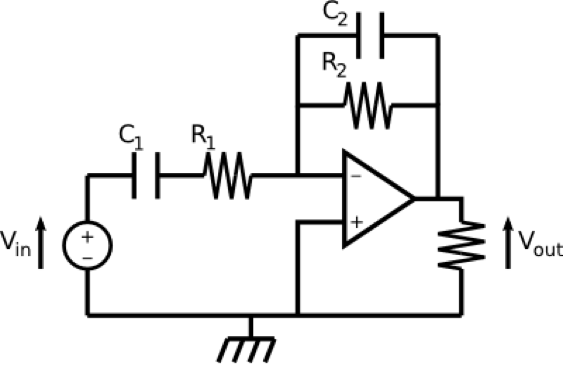
\includegraphics[width=6cm]{fig/circuit.png}
  \caption{A circuit with an operational amplifier.}
  \label{fig:circuit}
\end{figure}

After some circuit calculations (see MA2009), the transfer function
of this circuit can be determined as
\[
G(j\omega) = \frac{V_\textrm{out}}{V_\textrm{in}} = 
-\frac{R_2}{R_1}\frac{j\frac{\omega}{\omega_1}}
{\left(1+j\frac{\omega}{\omega_1}\right)\left(1+j\frac{\omega}{\omega_2}\right)},
\]
where
\[
\omega_1=\frac{1}{R_1C_1}, \quad \omega_2=\frac{1}{R_2C_2}.
\]

The Bode plots of this circuit (with $R_1=1\Omega, R_2=10\Omega,
C_1=1\textrm{mF}, C_2=1\mu\textrm{F}$) can then be obtained as below


\begin{figure}[H]
  \centering
  \includegraphics[width=11cm]{fig/circuit-bode.pdf}
  \caption{Bode plot of the circuit. The black vertical lines indicate
  the positions of $\omega_1=10^3$ and $\omega_2=10^5$.}
  \label{fig:circuit-bode}
\end{figure}

One can observe, in the gain plot, that the gain is maximal for
$\omega\in[\omega_1,\omega_2]$. Outside of that range, for
$\omega\to 0$ and $\omega\to\infty$, the gain decreases quickly and
converges to 0. Thus, one can say that the circuit is a
\emph{band-pass} filter, with the passband being
$[\omega_1,\omega_2]$.

Low-pass and high-pass filters can be similarly conveniently
visualized by their Bode plots.

\begin{figure}[H]
  \centering
  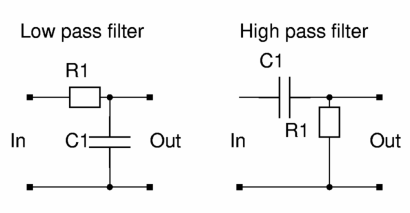
\includegraphics[width=12cm]{fig/low_high.png}\\
  \includegraphics[width=6cm]{fig/bode-low-pass.pdf}
  \includegraphics[width=6cm]{fig/bode-high-pass.pdf}
  \caption{Low and high pass filters and their Bode plots. The cut-off
    frequency is $\omega=0.1$ for both circuits.}
  \label{fig:low_high}
\end{figure}


\section{Bode plots : sketching}
\label{sec:bode-sketch}

\subsection{Properties}

Consider two systems with transfer functions $G(s)$ and $H(s)$. Remark
that
\[
20\log(\|G(j\omega)H(j\omega)\|) = 20\log(\|G(j\omega)\|) + 20 \log(\|H(j\omega)\|),
\]
\[
\angle(G(j\omega)H(j\omega)) = \angle(G(j\omega)) + \angle(H(j\omega)).
\]
Thus, the Bode plots of $G(s)H(s)$ can be obtained by \emph{adding}
those of $G(s)$ and $H(s)$. In practice, to sketch the Bode plots of a
complex function, we can
\begin{itemize}
\item decompose the complex function into a product of basic functions;
\item sketch the Bode plots of the basic functions;
\item add the Bode plots of the basic functions to obtain those of the
  original function.
\end{itemize}

Another interesting point to remark is that
\[
20\log\left(\left\|\frac{1}{G(j\omega)}\right\|\right) = -20\log(\|G(j\omega)\|),
\]
\[
\angle\left(\frac{1}{G(j\omega)}\right) = -\angle(G(j\omega)).
\]
Thus, the Bode plots of $1/G(s)$ can be obtained by flipping that of
$G(s)$ with respect to the X-axis.

\subsection{Bode plots of basic functions}

In this section, we shall designate by $y$ the coordinate of the
Y-axis and $x$ the log-coordinate of the X-axis,
i.e. $x=\log(\omega)$. Thus, a straight line in the Bode plot of the
amplitude will have equation $y=ax+b$.

\subsubsection{Constant terms}

For a constant real positive gain $K$, $20\log(|K|)$ is a constant
independent of $\omega$, so the amplitude plot is a horizontal line
with $y=20\log(|K|)$. Note that
\begin{itemize}
\item $y>0$ if $K>1$;
\item $y=0$ if $K=1$;
\item $y<0$ if $K<1$.
\end{itemize}

Next, $\angle K=0$, thus the phase plot is a horizontal line with
$y=0$. Fig.~\ref{fig:bode-const} shows the Bode plots for two values
of $K$.

\begin{figure}[H]
  \centering
  \includegraphics[width=12cm]{fig/bode-const.pdf}
  \caption{Bode plots for constant gains.}
  \label{fig:bode-const}
\end{figure}

\subsubsection{Derivative and integral terms}

Consider the derivative term $G(s)=s$. 
\begin{itemize}
\item We have
  $20\log(\|G(j\omega)\|)=20\log(\|j\omega\|)=20\log(\omega)$. Thus
  the Bode plot of the gain is a straight line with slope $+20$: every
  decade, the line goes up 20\,dB. For $\omega=1$, we have
  $20\log(\omega)=0$, so the line goes through the point
  $(x,y)=(0,0)$;
\item We have $\angle G(j\omega)=\angle j=\pi/2$. Thus the Bode plot
  of the phase is a horizontal line with $y=\pi/2$.
\end{itemize}

The Bode plots of the integral term $G(s)=1/s$ are the symmetric of
those of the derivative terms with respect to $y=0$. In particular
\begin{itemize}
\item The gain plot is a straight line with slope $-20$;
\item The phase plot is a horizontal line with $y=-\pi/2$.
\end{itemize}

Fig.~\ref{fig:bode-di} shows the Bode plots of the derivative and
integral terms.

\begin{figure}[H]
  \centering
  \includegraphics[width=12cm]{fig/bode-di.pdf}
  \caption{Bode plots for derivative and integral terms.}
  \label{fig:bode-di}
\end{figure}


\subsubsection{First-order terms}

Consider the transfer function $G(s)=s+a$. Regarding the gain plot,
\begin{itemize}
\item when $\omega\to 0$, $20\log(\|j\omega+a\|)\simeq
  20\log(a)$. Thus the asymptote to the left is a horizontal line
  with $y=20\log(a)$;
\item when $\omega\to\infty$, $20\log(\|j\omega+a\|)\simeq
  20\log(\|j\omega\|)=20\log(\omega)$. Thus, the asymptote to the
  right is a straight line with slope $+20$ (equation $y=20x$);
\item the two asymptotes meet when $20\log(a)=20x$,
  i.e. $\log(a)=x=\log(\omega)$, i.e. $\omega=a$. This intersection
  frequency $\omega=a$ is called the \emph{corner frequency}.
\end{itemize}

Regarding the phase plot
\begin{itemize}
\item when $\omega\to 0$, $\angle(j\omega+a) \simeq \angle a =
  0$. Thus the asymptote to the left is a horizontal line with $y=0$;
\item when $\omega\to\infty$, $\angle(j\omega+a) \simeq \angle j\omega
  = \pi/2$. Thus, the asymptote to the right is a horizontal line with
  $y=\pi/2$;
\item the transition occurs around the corner frequency $\omega=a$.
\end{itemize}

The Bode plots of $G(s)=1/(s+a)$ are the symmetric of those of the
derivative terms with respect to $y=0$. In particular
\begin{itemize}
\item the gain plot follows a horizontal asymptote $y=-\log(a)$ on the
  left, and a inclined asymptote with slope $-20$ on the right. The
  two asymptotes meet at the corner frequency $\omega=a$;
\item the phase plot follows a horizontal asymptote $y=0$ on the left,
  and a horizontal asymptote $y=-\pi/2$ on the right. The transition
  occurs around the corner frequency $\omega=a$.
\end{itemize}

Fig.~\ref{fig:bode-1st} shows the Bode plots for $G(s) = s+a$ and
$G(s)=1/(s+a)$ with $a=0.1$.

\begin{figure}[H]
  \centering
  \includegraphics[width=11cm]{fig/bode-first.pdf}
  \caption{Bode plots for first-order terms $G(s) = s+a$ and
    $G(s)=1/(s+a)$ with $a=0.1$. The corner frequency $\omega=a$ is
    indicated by a vertical dashed-dotted black line.}
  \label{fig:bode-1st}
\end{figure}


\subsubsection{Second-order terms}

Typical second-order terms we shall encounter have the following form  
\[
G(s) = \frac{\omega_n^2}{s^2+2\zeta\omega_ns+\omega_n^2}.
\]

Note that changing the term $\omega_n^2$ in the numerator to another
constant does not change the shape of the curve but will only shift
the curve up or down. However, it is important to scale the
second-order term $s^2+2\zeta\omega_ns+\omega_n^2$ so that the leading
coefficient is 1.

After dividing the numerator and the denominator by $\omega_n^2$, we
have
\[
G(j\omega) = \frac{1}{1-\frac{\omega^2}{\omega_n^2} +2j\zeta\frac{\omega}{\omega_n}}.
\]
Note that 
\begin{itemize}
\item when $\omega\to 0$, we have $\frac{\omega}{\omega_n} \to 0$,
  thus, $G(j\omega)\to 1$;
\item when  $\omega\to\infty$, 1 and $2j\zeta\frac{\omega}{\omega_n}$
  are negligible compared to $\frac{\omega^2}{\omega_n^2}$, thus
    $G(j\omega)\simeq -\frac{\omega_n^2}{\omega^2}$.
\end{itemize}

The above analysis leads to the following observations regarding the
gain plot
\begin{itemize}
\item the asymptote on the left is a horizontal line with $y=0$;
\item on the right, we have 
  \[
  20\log(\|G(j\omega\|)\simeq20\log(\omega_n^2/\omega^2)=40(\log(\omega_n)-\log(\omega)).
  \]
  Thus, the asymptote is a line with equation $y=40\log(\omega_n)-x$.
\item The two asymptotes meet when $0=40\log(\omega_n)-x$, i.e. when
  $\omega=\omega_n$. Thus $\omega_n$ is the corner frequency.
\end{itemize}

Regarding the phase plot, 
\begin{itemize}
\item the asymptote on the left is a horizontal line with $y=0$;
\item the asymptote on the right is a horizontal line with $y=-\pi$;
\item the transition occurs around the corner frequency $\omega=\omega_n$.
\end{itemize}


Fig.~\ref{fig:bode-2nd} shows the Bode plots of second-order terms for
different values of $\zeta$. Note that, while $\zeta$ has no influence
on the asymptotes, it affects the transition around the corner
frequency
\begin{itemize}
\item low values of $\zeta$ ($\zeta<0.707$) yield a peak in the gain
  plot (the smaller $\zeta$, the higher the peak) and a sharp decrease
  in the phase plot around the corner frequency;
\item high values of $\zeta$ ($\zeta>0.707$) yield a monotonically
  decreasing gain and a slow decrease in the phase plot around the
  corner frequency.
\end{itemize}

\begin{figure}[H]
  \centering
  \includegraphics[width=12cm]{fig/bode-second.pdf}
  \caption{Bode plots for second-order terms for $\omega_n=10$
    (indicated by a vertical dashed-dotted black line) and for
    different values of $\zeta$.}
  \label{fig:bode-2nd}
\end{figure}

\subsection{Bode plots of complex functions}
\label{sec:bode-complex}

As mentioned previously, one may sketch the Bode plots complex
function by
\begin{itemize}
\item decomposing the complex function into a product of basic functions;
\item sketching the Bode plots of the basic functions;
\item adding the Bode plots of the basic functions to obtain those of the
  original function.
\end{itemize}

However, the above approach can be tedious. Here we present another
approach, which is simpler but which requires more function
evaluations. In this approach, a Bode plot (gain or phase) is composed
of three parts:
\begin{enumerate}
\item Left part : from $\omega \simeq 0$ to
  $\omega=0.1\omega_{\min}$ where $\omega_{\min}$ is the smallest
  corner frequency. In this part, the plots will be represented by their
  left asymptotes;
\item Middle part : from $\omega=0.1\omega_{\min}$ to
  $\omega=10\omega_{\max}$ where $\omega_{\max}$ is the largest corner
  frequency. In this part, the plots will be constructed by sampling
  and numerical evaluations;
\item Right part : from $\omega=10\omega_{\max}$ to
  $\omega\simeq\infty$. In this part, the plots will be represented by
  their right asymptotes.
\end{enumerate}

\subsubsection{Left asymptotes}

Assume that the system is of type $k$, i.e.
\[
G(s) = \frac{N(s)}{s^kD(s)},
\]
with $N(0)\neq 0$ and $D(0)\neq 0$. Note that we are interested in the
function $G$ itself, not the corresponding unity-feedback function
$G/(1+G)$. 

Regarding the gain plot, we have, when $\omega\to 0$
\[
20\log(\|G(j\omega)\|) \simeq
20\log\left(\frac{|N(0)|}{\omega^k|D(0)|}\right)
= 20\log\left(\frac{|N(0)|}{|D(0)|}\right) - 20k\log(\omega).
\]

Thus, the asymptote on the left will be straight line with slope
$-20k$\,dB/decade. To find one point on this line, we may evaluate
the equation of the line at e.g. $\omega=1$, to find that the line
must pass through $(x,y)=(0,20\log(|N(0)/D(0)|)$. Note that the
asymptote might stop before $\omega=1$ in case $\omega_{\min} < 1$.

Regarding the angle plot, we have, when $\omega\to 0$
\[
\angle G(j\omega) \simeq \angle(N(0)/D(0)) - k\angle(j\omega).
\]
Thus, 
\begin{itemize}
\item if $N(0)/D(0)>0$, we have a horizontal asymptote with
$y=-k\pi/2 \mod 2\pi$;
\item  if $N(0)/D(0)<0$, we have a horizontal asymptote with
$y=\pi-k\pi/2\mod 2\pi$.
\end{itemize}

\subsubsection{Right asymptotes}

Assume that the system is of order $n$, i.e.
\[
G(s) = \frac{N(s)}{D(s)},
\]
with $\deg(D)-\deg(N)=n$. Note that we are interested in the
function $G$ itself, not the corresponding unity-feedback function
$G/(1+G)$. 

Regarding the gain plot, we have, when $\omega\to \infty$
\[
20\log(\|G(j\omega)\|) \simeq
20\log\left(\frac{|A|}{\omega^n}\right)
= 20\log |A| - 20n\log(\omega),
\]
where $A$ is the ratio of the leading coefficient of $N$ to the
leading coefficient of $D$. Thus, the asymptote on the right will be
straight line with slope $-20n$\,dB/decade. To find one point on this
line, we may evaluate the equation of the line at e.g. $\omega=1$, to
find that the line must pass through $(x,y)=(0,20\log |A|)$. Note that
the asymptote might stop before $\omega=1$ in case $\omega_{\max} >
1$.

Regarding the angle plot, we have, when $\omega\to \infty$
\[
\angle G(j\omega) \simeq \angle A - n\angle(j\omega).
\]
Thus, 
\begin{itemize}
\item if $A>0$, we have a horizontal asymptote with
$y=-n\pi/2 \mod 2\pi$;
\item  if $A<0$, we have a horizontal asymptote with
$y=\pi-n\pi/2\mod 2\pi$.
\end{itemize}


\subsubsection{Middle part}

The middle part ranges from $\omega=0.1\omega_{\min}$ to
$\omega=10\omega_{\max}$. Here, we simply \emph{sample} some points in
the interval $(0.1\omega_{\min},10\omega_{\max})$ and evaluate
\emph{numerically} $20\log(\|G(j\omega)\|)$ and $\angle
G(j\omega)$. Since the plots tend to display large variations around
the corner frequencies, we shall sample more densely around the corner
frequencies.

\begin{example}
  \label{ex:bode-sketch}
  Let us sketch the Bode plots of the transfer function
  \[
  G(s) = \frac{-5(s+0.1)}{s^2(s^2+0.1s+49)}
  \]

  \begin{description}
  \item[Step 1] Identify the corner frequencies:
    \begin{itemize}
    \item the first-order term $s+0.1$ has a corner frequency at
      $\omega=0.1$;
    \item the second-order term $s^2+0.1s+49$ has a corner frequency at
      $\omega=\sqrt{49}=7$. 
    \end{itemize}
    Thus, $\omega_{\min}=0.1$ and $\omega_{\max}=7$.
  \item[Step 2] Left part. We have a term $1/s^2$, thus system type is
    $2$. The gain plot therefore has a left asymptote with slope
    $-40$\,dB/decade and going through the point
    \[
    (x,y)=\left(0,20\log\left(\frac{0.5}{49}\right)\right)=(0,-39.82).
    \]
    The phase plot has a horizontal left asymptote with 
    \[
    y=\pi-2*\frac{\pi}{2}= 0.
    \]
  \item[Step 3] Right part. The numerator has degree 1 and the
    denominator has degree 4, thus the system order is $4-1=3$. The
    gain plot therefore has a right asymptote with slope
    $-60$\,dB/decade. The leading coefficient of the numerator is
    $-5$, the leading coefficient of the denominator is $1$, thus
    $A=-5$. The right asymptote thus goes through the point
    \[
    (x,y)=(0,20\log 5)=(0,13.98).
    \]
    The phase plot has a horizontal right asymptote with 
    \[
    y=\pi-3*\frac{\pi}{2}= -\frac{\pi}{2}.
    \]
  \item[Step 4] Middle part. We sample the $X$-axis for
    $\omega\in(0.01,70)=(10^{-2},10^{1.85})$.
    
  \begin{tabular}{|r|r|r|r|}
    \hline
    $x$ & $\omega$ & $20\log(\|G(j\omega)\|)$ & $\angle G(j\omega)$\\
    \hline
    -2 & 0.01 & 40.22 & 0.1 \\
    -1.5 & 0.03 & 20.59 & 0.31 \\
    -1 & 0.1 & 3.19 & 0.79 \\
    -0.5 & 0.32 & -9.39 & 1.26 \\
    0 & 1.0 & -19.6 & 1.47 \\
    0.5 & 3.16 & -27.84 & 1.53 \\
    1 & 10.0 & -40.17 & -1.56 \\
    1.5 & 31.62 & -75.58 & -1.57 \\
    1.85 & 70.79 & -96.94 & -1.57 \\
    \hline
  \end{tabular}

  Now, we sample more densely around $\omega=0.1$ and $\omega=7$.

  \begin{tabular}{|r|r|r|r|}
    \hline
    $x$ & $\omega$ & $20\log(\|G(j\omega)\|)$ & $\angle G(j\omega)$\\
    \hline
    -1.15 & 0.07 & 7.94 & 0.62 \\
    -1.1 & 0.08 & 6.3 & 0.67 \\
    -1.05 & 0.09 & 4.72 & 0.73 \\
    -1 & 0.1 & 3.19 & 0.79 \\
    -0.95 & 0.11 & 1.72 & 0.84 \\
    -0.9 & 0.13 & 0.3 & 0.9 \\
    -0.85 & 0.14 & -1.06 & 0.95 \\
    \hline
  \end{tabular}

  \begin{tabular}{|r|r|r|r|}
    \hline
    $x$ & $\omega$ & $20\log(\|G(j\omega)\|)$ & $\angle G(j\omega)$\\
    \hline
    0.7 & 5.01 & -27.58 & 1.53 \\
    0.75 & 5.62 & -25.82 & 1.52 \\
    0.8 & 6.31 & -21.31 & 1.49 \\
    0.85 & 7.08 & -5.46 & -1.02 \\
    0.9 & 7.94 & -27.02 & -1.53 \\
    0.95 & 8.91 & -34.69 & -1.55 \\
    1 & 10.0 & -40.17 & -1.56 \\
    \hline
  \end{tabular}

  \item[Step 5] We can now sketch the Bode plots in
    Fig.~\ref{fig:bode-complex}. For $\omega<0.01$, we use the left
    asymptotes (both gain and phase plots). For $\omega\in(0.01,70)$,
    we use the sampled points joined by straight segments. For
    $\omega>70$, we use the right asymptotes.

  \begin{figure}[H]
    \centering
    \includegraphics[width=12cm]{fig/bode-complex.pdf}
    \caption{Bode plots for a complex function. The exact Bode plots
      are in bold light gray. The asymptotes are in dashed blue. The
      sampled points are green and joined by green segments. We can
      see that the plots sketched by the method presented previously
      approximate quite well the exact Bode plots.}
    \label{fig:bode-complex}
  \end{figure}
  \end{description}
\end{example}

\section{Bode plots : analysis}
\label{sec:bode-analysis}

Assume now that we are given a system but that we do not know its
transfer function. We can subject the system to sinusoidal inputs of
various frequencies and report the amplitude of the system
responses. Doing so will enable us to \emph{experimentally} sketch the
Bode plot of the gain of the system.

Next, from this experimental Bode plot, we can reverse-engineer some
important information about the system itself.

\subsection{Determining system type and system order}

In Section~\ref{sec:bode-complex}, we found that a system of type $k$
has a left asymptote with slope $-20k$\,dB/decade. Thus, from the
experimental the Bode plot of the gain, we can
\begin{itemize}
\item fit a straight line to the \emph{extreme left} portion of the
  plot;
\item compute the slope $\sigma_\mathrm{left}$ of this line;
\item obtain the system type by rounding $-\sigma_\mathrm{left}/20$
  to the closest integer.
\end{itemize}

Similarly, regarding the system order, we can
\begin{itemize}
\item fit a straight line to the \emph{extreme right} portion of the
  gain plot;
\item compute the slope $\sigma_\mathrm{right}$ of this line;
\item obtain the system type by rounding $-\sigma_\mathrm{right}/20$
  to the closest integer.
\end{itemize}

\subsection{Determining position and velocity constants and steady-state
  errors}
\label{sec:errors}

\subsubsection{Type-0 systems}

Assume that we have determined that a given system is of type 0, (in
other words, we have found that the gain plot has a horizontal left
asymptote). If the transfer function of the system is $G$, then the
Y-coordinate of this asymptote is given by
\[
\lim_{\omega\to 0} 20\log(\|G(j\omega)\|) = 20\log(|G(0)|) = 20\log K_p,
\]
where $K_p$ is the position constant. Thus, we can find the position
constant of a type-0 system as follows
\begin{itemize}
\item denote by $y_\mathrm{asymptote}$ the Y-coordinate of the horizontal
  left asymptote;
\item compute $K_p$ by $K_p = 10^{\frac{y_\mathrm{asymptote}}{20}}$.
\end{itemize}

Finally, we can also compute the steady-state error to step input of
the corresponding unity-feedback system (whose TF is $G/(1+G)$) by
\[
e_{ss} = \frac{1}{1+K_p}.
\]

\begin{example}
  \label{ex:bode-type0}
  We have experimentally determined the gain plot of a system with
  unknown transfer function in Fig.~\ref{fig:bode-type0}.
  \begin{figure}[H]
    \centering
    \includegraphics[width=10cm]{fig/bode-type0.pdf}
    \caption{Gain plot of a system with unknown transfer
      function. Straight lines (green dashed and blue dashed-dotted)
      are fitted to the extreme left and right portions of the plot.}
    \label{fig:bode-type0}
  \end{figure}

  The left asymptote is horizontal, indicating a system type
  $k=0$. The right asymptote has a slope of $-20$\,dB/decade,
  indicating a system order $n=1$.

  Next, since the system is of type 0, we can calculate the position
  constant $K_p$. We determine graphically that the Y-coordinate of
  the horizontal asymptote is $y_\mathrm{asymptote}\simeq
  -68$\,dB. Thus, the position constant is given by
  \[
  K_p \simeq 10^{-68/20}  \simeq 0.0004.
  \]

  Finally, the steady-state error to unit step input of the
  corresponding unity-feedback system is
  \[
  e_{ss} = \frac{1}{1+K_p} \simeq 1.
  \]


\end{example}

\subsubsection{Type-1 systems}

Assume that we have determined that a given system is of type 1, (in
other words, we have found that the gain plot has a left asymptote
with slope $-20$\,dB/decade). Thus, the transfer function of the
system has the form
\[
G(s) = \frac{N(s)}{sD(s)},
\]
with $N(0)\neq 0$ and $D(0)\neq 0$. Next, the velocity constant of the
system is given by
\[
K_v = \frac{|N(0)|}{|D(0)|}.
\]
On the other hand, we noted in Section~\ref{sec:bode-complex} that the
left asymptote goes through the point
$(x,y)=(0,20\log(|N(0)/D(0)|)$. Thus, we can find the velocity
constant of a type-1 system as follows
\begin{itemize}
\item determine the intersection of the left asymptote with the
  vertical line $x=0$ (or $\omega=1$) and denote by
  $y_\mathrm{intersect}$ the Y-coordinate of this intersection;
\item compute $K_v$ by $K_v = 10^{\frac{y_\mathrm{intersect}}{20}}$.
\end{itemize}

Finally, we can also compute the steady-state error to ramp input of
the corresponding unity-feedback system (whose TF is $G/(1+G)$) by
\[
e_{ss} = \frac{1}{K_v}.
\]

\begin{example}
  \label{ex:bode-type1}
  We have experimentally determined the gain plot of a system with
  unknown transfer function in Fig.~\ref{fig:bode-type1}.
  \begin{figure}[H]
    \centering
    \includegraphics[width=10cm]{fig/bode-type1.pdf}
    \caption{Gain plot of a system with unknown transfer
      function. Straight lines (green dashed and blue dashed-dotted)
      are fitted to the extreme left and right portions of the plot.}
    \label{fig:bode-type1}
  \end{figure}

  The left asymptote has a slope of $-20$\,dB/decade, indicating a
  system type $k=1$. The right asymptote is horizontal, indicating a
  system order $n=0$.

  Next, since the system is of type 1, we can calculate the velocity
  constant $K_v$. We determine graphically that the left asymptote
  intersects the vertical line $x=0$ (or $\omega=1$) at a point with
  Y-coordinate $y_\mathrm{intersect}\simeq -26$\,dB. 
  Thus, the velocity constant is given by
  \[
  K_v \simeq 10^{-26/20}  \simeq 0.05.
  \]

  Finally, the steady-state error to unit ramp input of the
  corresponding unity-feedback system is
  \[
  e_{ss} = \frac{1}{K_v} \simeq 20.
  \]
\end{example}

\subsection{Stability margins}
\label{sec:margins}

\subsubsection{Nyquist stability criterion}

In the the previous section, we showed that the Bode plots of an
open-loop system can give information about the \emph{steady-state
  errors} of the corresponding unity-feedback system. Here, we show
how the open-loop Bode plots can also tell us whether the
corresponding unity-feedback system is \emph{stable}. This is done
through the following theorem

\begin{theorem}[Nyquist stability criterion]
  Consider a stable system with transfer function $G$. The
  corresponding unity-feedback system (whose transfer function is
  $G/(1+G)$) is stable if and only if
  \begin{equation}
    \label{eq:nyq}
    \|G(j\omega)\| < 1\quad \textrm{when}\quad \angle G(j\omega) = \pm\pi
    \mod 2\pi.  
  \end{equation}
  An equivalent condition is
  \begin{equation}
    \label{eq:nyq2}
    \angle G(j\omega) > -\pi \quad \textrm{when}\quad
    \|G(j\omega)\| = 1.  
  \end{equation}
\end{theorem}


\begin{example}
  \label{ex:nyq}
  Consider a system with transfer function 
  \[
  G=\frac{200}{(s+2)(s+4)(s+5)}.
  \]
  The Bode plots of this system is presented in
  Fig.~\ref{fig:bode-nyq}, red plain lines.
  \begin{figure}[H]
    \centering
    \includegraphics[width=12cm]{fig/bode-nyq.pdf}
    \caption{Nyquist criterion (gain condition).}
    \label{fig:bode-nyq}
  \end{figure}

  Let us determine whether the corresponding unity-feedback system is
  stable using the (first) Nyquist criterion~\ref{eq:nyq}. From the
  phase plot, we can see that $\angle G(j\omega) = -\pi$ for
  $\omega\simeq 6.6$\,rad/s. Consider now the gain plot. At
  $\omega=6.6$\,rad/s, we find that the gain in dB is \emph{negative}
  (around -5.5\,dB), which means that $\|G(j\omega)\|<1$. Therefore,
  we can conclude that the corresponding unity-feedback system is
  \emph{stable}.

  Consider a system with transfer function 
  \[
  G_2=\frac{600}{(s+2)(s+4)(s+5)}.
  \]
  The Bode plots of this system is presented in
  Fig.~\ref{fig:bode-nyq}, green dashed lines. From the phase plot, we
  can see that $\angle G_2(j\omega) = -\pi$ for $\omega\simeq
  6.6$\,rad/s (same as for the previous system, since the constant
  gains -- 600 or 200 -- do not contribute to the phase). In the gain
  plot, we find that the gain in dB at $\omega\simeq 6.6$ is
  \emph{positive} (around +4\,dB), which means that
  $\|G_2(j\omega)\|>1$. Therefore, we can conclude that the
  corresponding unity-feedback system is \emph{unstable}.
\end{example}

\begin{example}
  \label{ex:nyq2}
  Consider again the system with transfer function 
  \[
  G=\frac{200}{(s+2)(s+4)(s+5)}.
  \]
  The Bode plots of this system is presented in
  Fig.~\ref{fig:bode-nyq}, red plain lines.
  \begin{figure}[H]
    \centering
    \includegraphics[width=12cm]{fig/bode-nyq2.pdf}
    \caption{Nyquist criterion (phase condition).}
    \label{fig:bode-nyq2}
  \end{figure}

  Let us determine whether the corresponding unity-feedback system is
  stable using the (second) Nyquist criterion~\ref{eq:nyq}. From the
  phase plot, we can see that $\|G(j\omega)\| = 1$ for $\omega\simeq
  4.5$\,rad/s. Consider now the phase plot. At $\omega=4.5$\,rad/s, we
  find that the phase is $\angle G(j\omega)\simeq
  -2.7>-\pi$. Therefore, we can conclude that the corresponding
  unity-feedback system is \emph{stable}.

  Consider the system with transfer function 
  \[
  G_2=\frac{600}{(s+2)(s+4)(s+5)}.
  \]
  The Bode plots of this system is presented in
  Fig.~\ref{fig:bode-nyq}, green dashed lines. From the phase plot, we
  can see that the $\|G_2(j\omega_2)\| = 1$ for $\omega_2\simeq
  7.5$\,rad/s. In the phase plot, we find that $\angle
  G_2(j\omega_2)\simeq -3.35<-\pi$. Therefore, we can conclude that
  the corresponding unity-feedback system is \emph{unstable}.
\end{example}



% \textbf{Proof\quad} Assume that $G=N/D$. Consider the root locus of
% the system

% \begin{figure}[H]
%   \label{fig:simple}
%   \centering
%   \tikzstyle{block} = [draw, fill=blue!20, rectangle, minimum height=3em, minimum width=4em]
%   \tikzstyle{controller} = [draw, fill=red!20, rectangle, minimum height=3em, minimum width=4em]
%   \tikzstyle{sum} = [draw, fill=blue!20, circle, node distance=1cm]
%   \tikzstyle{input} = [coordinate]
%   \tikzstyle{output} = [coordinate]
%   \begin{tikzpicture}[auto, >=latex']
%     Nodes
%     \node [input] (input) {};
%     \node [sum, right = 0.5cm of input] (sum) {};
%     \node [block, right = 0.5cm of sum] (system) {$K\frac{N}{D}$};
%     \node [output, right = 1cm of system] (output) {};
%     \node [input, below = 0.5cm of system] (m) {};
%     Arrows
%     \draw [draw,->] (input) -- node {$R$} (sum);
%     \draw [->] (sum) -- node {} (system);
%     \draw [->] (system) -- node (y) {$C$}(output);
%     \draw [-] (y) |- (m) {} ;
%     \draw [->] (m) -| node[pos=0.99] {$-$}  node [near end] {} (sum);
%   \end{tikzpicture}  
% \end{figure}

% The transfer function of this system is
% \[
% \frac{C}{R} = \frac{KN}{N+KD}.
% \]

% The 

% $\Box$

\subsubsection{Gain margin and phase margin}

We have seen in Example~\ref{ex:nyq} that increasing the gain of the
open-loop TF from 200 to 600 made the corresponding unity-feedback
system become unstable. Can we determine from the Bode plots the
\emph{maximum} gain increase before the corresponding unity-feedback
system becomes unstable ?

The answer is yes. Consider again the TF
\[
G=\frac{200}{(s+2)(s+4)(s+5)}.
\]
We saw that the frequency for which $\angle G(j\omega) = -\pi$ was
$\omega\simeq 6.6$\,rad/s. Next, the gain at this frequency was found
to be $20\log\|G(j\omega)\|=-5.5$\,dB.

Assume now that the TF has been multiplied by a factor $K$, so that
the new TF is
\[
KG = \frac{200K}{(s+2)(s+4)(s+5)}.
\]
We have $\angle KG$ = $\angle G$, so $\angle KG(j\omega) = -\pi$ also for
$\omega\simeq 6.6$\,rad/s. Next, the gain at this frequency will be
\[
20\log\|KG(j\omega)\| = 20\log K + 20\log\|G(j\omega)\|= 20\log K -5.5\,\mathrm{dB}.
\]
If we want the unity-feedback system associated with $KG$
to be stable, we must have, by the Nyquist criterion
\[
20\log\|KG(j\omega)\| < 0,
\]
which implies that $20\log K<5.5$\,dB (or $K< 10^{5.5/20}=1.88$).

The value $G_M=5.5\,dB$ is called the \emph{gain margin} of system
$G$: if we multiply $G$ by a factor $K$ such that $20\log K<G_M$, then
the corresponing unity-feedback system remains stable ; if we multiply
$G$ by a factor $K$ such that $20\log K>G_M$, then the corresponing
unity-feedback system will become unstable. 

To verify the latter assertion, consider again the transfer function
$G_2=\frac{600}{(s+2)(s+4)(s+5)}$. Remark that $G_2=3G$. Next, $20\log
3=9.54>5.5$. Thus, $G$ has been increased by a factor larger than the
gain margin, which implies that the unity-feedback system
corresponding to $G_2$ will be unstable. This is confirmed by
Example~\ref{ex:nyq}.

In general, we can see from the above development that the gain margin
is given by $G_M=-20\log\|G(j\omega^*)\|$ where $\omega^*$ is the
frequency that verifies $\angle
G(j\omega^*)=-\pi$. Fig.~\ref{fig:bode-gain-margin} illustrates the
evaluation of $G_M$ for $G=\frac{200}{(s+2)(s+4)(s+5)}$.
\begin{figure}[H]
  \centering
  \includegraphics[width=10cm]{fig/bode-gain-margin-mod.pdf}
  \caption{Gain margin for $G=\frac{200}{(s+2)(s+4)(s+5)}$.}
  \label{fig:bode-gain-margin}
\end{figure}

Similarly, one can define the \emph{phase margin} $\phi_M$ as follows:
$\phi_M$ is the maximum angle that we can subtract to the open-loop
transfer function before the corresponding unity-feedback feedback
system becomes unstable. Formally, $\phi_M$ is given by
$\phi_M=\pi+\angle G(j\omega^*)$ where $\omega^*$ is the frequency
that verifies $\|G(j\omega^*)\|=1$.  For
$G=\frac{200}{(s+2)(s+4)(s+5)}$, Example~\ref{ex:nyq2} showed that
$\phi_M\simeq\pi-2.7\simeq 0.44$\,rad. Fig.~\ref{fig:bode-phase-margin}
illustrates this evaluation.

\begin{figure}[H]
  \centering
  \includegraphics[width=10cm]{fig/bode-phase-margin-mod.pdf}
  \caption{Phase margin for $G=\frac{200}{(s+2)(s+4)(s+5)}$.}
  \label{fig:bode-phase-margin}
\end{figure}

Large stability margins (both gain and phase margins) ensure that the
corresponding unity-feedback will be stable even if there are some
variations in the system components. One can also say, roughly, that
the larger the margins, the larger the damping (hence the more stable
the unity-feedback system). Usually, a gain margin of at least 6\,dB
and a phase margin of 30 to 60 degrees are required ($\simeq$ 0.5 to
1\,rad).


\subsection{Some remarks on controller design by the
  frequency-response method}

Section~\ref{sec:errors} and~\ref{sec:margins} have shown us how the
Bode plots of a system with transfer function $G$ can give us
information about the corresponding unity-feedback system (whose
transfer function is $G/(1+G)$):
\begin{itemize}
\item Section~\ref{sec:errors} showed that the asymptotic behavior of
  $G$ when $\omega\to 0$ can give information about the
  steady-state error to step inputs (type~0 system) or to ramp inputs
  (type~1 systems) of the corresponding unity-feedback system;
\item Section~\ref{sec:margins} showed how to compute stability
  margins from the Bode plots of $G$, which give us information about
  the stability of the corresponding unity-feedback system.
\end{itemize}

In turn, this information can be used in controller design. Consider
for instance the system of Example~\ref{ex:bode-type1}. We determined
that its velocity constant was $K_v=0.05$, which yields a steady-state
error of the corresponding unity-feedback system to unit ramp input of
$e_{ss}=20$. If we want to decrease the steady-state error to
one-tenth of this value (without considering the change in the
transient behavior), we can for instance use a gain adjustment method
whereby we would multiply the open-loop TF by a factor 10, which would
result in $K_v^\textrm{new}=0.5$, and
$e_{ss}^\textrm{new}=1/K_v^\textrm{new}=2$.

The stability margins can be used in compensator design. Basically, we
have seen in Section~\ref{sec:lead} that a lead compensator ``added
phase'' to the system. Thus, one can improve the stability of a system
(i.e. achieving larger phase margin) by adding a lead compensator that
contribute the appropriate amount of phase. However, in practice, the
design of lead/lag compensators is relatively involved, so it will not
be covered here.


% \bibliographystyle{apalike}
% \bibliography{../../cri}


\end{document}



%%%LocalVariables:
%%%mode:latex
%%%TeX-master:t
%%%End:
